%%%%%% Run at command line, run
%%%%%% xelatex grad-sample.tex 
%%%%%% for a few times to generate the output pdf file
\documentclass[12pt,oneside,openright,a4paper]{cpe-english-project}
\usepackage{algorithm}
\usepackage{algpseudocode}
\usepackage{polyglossia}
\usepackage{tabularx}
\usepackage{array}
\usepackage{float}
\usepackage{placeins}
\usepackage{hyperref}
\setdefaultlanguage{english}
\setotherlanguage{thai}
\newfontfamily\thaifont[Script=Thai,Scale=1.23]{TH Sarabun New}
\defaultfontfeatures{Mapping=tex-text,Scale=1.0,LetterSpace=0.0}
\setmainfont[Scale=1.0,LetterSpace=0,WordSpace=1.0,FakeStretch=1.0]{Times New Roman}
\emergencystretch=10pt
%\XeTeXlinebreaklocale "th_TH"	
%\XeTeXlinebreakskip = 0pt plus 1pt
%\setmathfont(Digits)[Scale=1.0,LetterSpace=0,FakeStretch=1.0]{Times New Roman}


%%%%%%%%%%%%%%%%%%%%%%%%%%%%%%%%%%%%%%%%%%%%%%%%%%%%%%%%%%%%%%%%%%%
% Customize below to suit your needs 
% The ones that are optional can be left blank. 
%%%%%%%%%%%%%%%%%%%%%%%%%%%%%%%%%%%%%%%%%%%%%%%%%%%%%%%%%%%%%%%%%%%
% First line of title
\def\disstitleone{Generalizable Artificial Intelligence Agent in Game Development}   
% Second line of title
\def\disstitletwo{}   
% Your first name and lastname
\def\dissauthor{Mr. Tanatanee Ponark}   % 1st member
%%% Put other group member names here ..
\def\dissauthortwo{Mr. Intouch Yusoh}   % 2nd member (optional)
\def\dissauthorthree{}   % 3rd member (optional)


% The degree that you're persuing..
\def\dissdegree{Bachelor of Engineering} % Name of the degree
\def\dissdegreeabrev{B.Eng} % Abbreviation of the degree
\def\dissyear{2024}                   % Year of submission
\def\thaidissyear{2567}               % Year of submission (B.E.)

%%%%%%%%%%%%%%%%%%%%%%%%%%%%%%%%%%%%%%%%%%%%
% Your project and independent study committee..
%%%%%%%%%%%%%%%%%%%%%%%%%%%%%%%%%%%%%%%%%%%%
\def\dissadvisor{Assoc.Prof. Natasha Dejdumrong, D.Tech.Sci.}  % Advisor
%%% Leave it empty if you have no Co-advisor
\def\disscoadvisor{}  % Co-advisor
%%% Leave it empty if you have no Co-advisor 2
\def\disscoadvisortwo{}  % Co-advisor 2 (if any)
\def\disscoadvisorthree{}  % Co-advisor 3 (You better be building space rocket or curing cancer at this point)
\def\disscommitteetwo{Asst.Prof. Nuttanart Muansuwan, Ph.D.}  % 3rd committee member (optional)
\def\disscommitteethree{Asst.Prof. Phond Phunchongharn, Ph.D.}   % 4th committee member (optional) 
\def\disscommitteefour{Jaturon Harnsomburana, Ph.D.}    % 5th committee member (optional) 

\def\worktype{Project} %%  Project or Independent study
\def\disscredit{3}   %% 3 credits or 6 credits


\def\fieldofstudy{Computer Engineering} 
\def\department{Computer Engineering} 
\def\faculty{Engineering}

\def\thaifieldofstudy{วิศวกรรมคอมพิวเตอร์} 
\def\thaidepartment{วิศวกรรมคอมพิวเตอร์} 
\def\thaifaculty{วิศวกรรมศาสตร์}
 
\def\appendixnames{Appendix} %%% Appendices or Appendix

\def\thaiworktype{ปริญญานิพนธ์} %  Project or research project % 
\def\thaidisstitleone{ปัญญาประดิษฐ์ที่ปรับตัวได้สำหรับการพัฒนาเกม}
\def\thaidisstitletwo{}
\def\thaidissauthor{นายธนธานี โพธิ์นาค}
\def\thaidissauthortwo{นายอินทัช ยูโซะ} %Optional
\def\thaidissauthorthree{} %Optional

\def\thaidissadvisor{รศ.ดร.ณัฐชา เดชดำรง}
%% Leave this empty if you have no co-advisor
\def\thaidisscoadvisor{} %Optional
\def\thaidisscoadvisortwo{}  % Co-advisor 2 (if any)
\def\thaidisscoadvisorthree{} % Co-advisor 3 (You better be building space rocket or curing cancer at this point)
\def\thaidissdegree{วิศวกรรมศาสตรบัณฑิต}

% Change the line spacing here...
\linespread{1.15}

%%%%%%%%%%%%%%%%%%%%%%%%%%%%%%%%%%%%%%%%%%%%%%%%%%%%%%%%%%%%%%%%
% End of personal customization.  Do not modify from this part 
% to \begin{document} unless you know what you are doing...
%%%%%%%%%%%%%%%%%%%%%%%%%%%%%%%%%%%%%%%%%%%%%%%%%%%%%%%%%%%%%%%%


%%%%%%%%%%%% Dissertation style %%%%%%%%%%%
%\linespread{1.6} % Double-spaced  
%%\oddsidemargin    0.5in
%%\evensidemargin   0.5in
%%%%%%%%%%%%%%%%%%%%%%%%%%%%%%%%%%%%%%%%%%%
%\renewcommand{\subfigtopskip}{10pt}
%\renewcommand{\subfigbottomskip}{-5pt} 
%\renewcommand{\subfigcapskip}{-6pt} %vertical space between caption
%                                    %and figure.
%\renewcommand{\subfigcapmargin}{0pt}

\renewcommand{\topfraction}{0.85}
\renewcommand{\textfraction}{0.1}

\newtheorem{theorem}{Theorem}
\newtheorem{lemma}{Lemma}
\newtheorem{corollary}{Corollary}

\def\QED{\mbox{\rule[0pt]{1.5ex}{1.5ex}}}
\def\proof{\noindent\hspace{2em}{\itshape Proof: }}
\def\endproof{\hspace*{\fill}~\QED\par\endtrivlist\unskip}
%\newenvironment{proof}{{\sc Proof:}}{~\hfill \blacksquare}
%% The hyperref package redefines the \appendix. This one 
%% is from the dissertation.cls
%\def\appendix#1{\iffirstappendix \appendixcover \firstappendixfalse \fi \chapter{#1}}
%\renewcommand{\arraystretch}{0.8}
%%%%%%%%%%%%%%%%%%%%%%%%%%%%%%%%%%%%%%%%%%%%%%%%%%%%%%%%%%%%%%%%
%%%%%%%%%%%%%%%%%%%%%%%%%%%%%%%%%%%%%%%%%%%%%%%%%%%%%%%%%%%%%%%%


\begin{document}
\pdfstringdefDisableCommands{%
\let\MakeUppercase\relax
}
\begin{center}
  
\includegraphics[width=2.8cm]{logo02.jpg}
\end{center}
\vspace*{-1cm}

\maketitlepage
\makesignaturepage 

%%%%%%%%%%%%%%%%%%%%%%%%%%%%%%%%%%%%%%%%%%%%%%%%%%%%%%%%%%%%%%
%%%%%%%%%%%%%%%%%%%%%% English abstract %%%%%%%%%%%%%%%%%%%%%%%
%%%%%%%%%%%%%%%%%%%%%%%%%%%%%%%%%%%%%%%%%%%%%%%%%%%%%%%%%%%%%%
\abstract

In recent years, the application of artificial intelligence (AI) in game development has garnered significant attention, particularly in enhancing gameplay and automating testing processes. However, most existing AI systems are tailored for specific games or tasks, limiting their adaptability and reusability across different projects. This study proposes the development of an adaptive AI agent for 2D platformer games using reinforcement learning. The agent is trained within a Unity-based environment to learn essential player behaviors, such as movement, jumping, and obstacle avoidance. Leveraging the Proximal Policy Optimization (PPO) algorithm, the system is designed with modular components to promote flexibility, scalability, and ease of integration. By separating action execution from decision-making, the architecture facilitates the extension of the agent’s capabilities to support additional actions or mechanics. The trained AI model is packaged as a reusable Unity asset, intended for deployment in similar 2D games either as an intelligent NPC or an automated game tester. This approach aims to reduce development time and technical barriers for indie developers seeking to integrate intelligent behavior into their games. The results demonstrate the potential of reinforcement learning in constructing adaptable game agents and contribute toward making AI tools more accessible in the domain of game development.

\begin{flushleft}
\begin{tabular*}{\textwidth}{@{}lp{0.8\textwidth}}
\textbf{Keywords}: & Game Development / Artificial Intelligence / Enemy AI / Reusable Assets / Non-Player Characters / Adaptive AI / Reinforcement Learning / Procedural Learning / Game AI Training / AI Assets
\end{tabular*}
\end{flushleft}
\endabstract

%%%%%%%%%%%%%%%%%%%%%%%%%%%%%%%%%%%%%%%%%%%%%%%%%%%%%%%%%%%%%%
%%%%%%%%%% Thai abstract here %%%%%%%%%%%%%%%%%%%%%%%%%%%%%%%%%
%%%%%%%%%%%%%%%%%%%%%%%%%%%%%%%%%%%%%%%%%%%%%%%%%%%%%%%%%%%%%%
{
%\begin{thai}
\XeTeXlinebreaklocale "th_TH"	
\XeTeXlinebreakskip = 0pt plus 1pt
\thaifont
\thaiabstract

Thai translation coming soon

\begin{flushleft}
\begin{tabular*}{\textwidth}{@{}lp{0.8\textwidth}}
 & \\

\textbf{คำสำคัญ}: & Game Development / Artificial Intelligence / Enemy AI / Reusable Assets / Non-Player Characters / Adaptive AI / Reinforcement Learning / Procedural Learning / Game AI Training / AI Assets
\end{tabular*}
\end{flushleft}
\endabstract
%\end{thai}
}

%%%%%%%%%%%%%%%%%%%%%%%%%%%%%%%%%%%%%%%%%%%%%%%%%%%%%%%%%%%%
%%%%%%%%%%%%%%%%%%%%%%% Acknowledgments %%%%%%%%%%%%%%%%%%%%
%%%%%%%%%%%%%%%%%%%%%%%%%%%%%%%%%%%%%%%%%%%%%%%%%%%%%%%%%%%%
\preface
Acknowledge your advisors and thanks your friends here..

%%%%%%%%%%%%%%%%%%%%%%%%%%%%%%%%%%%%%%%%%%%%%%%%%%%%%%%%%%%%%
%%%%%%%%%%%%%%%% ToC, List of figures/tables %%%%%%%%%%%%%%%%
%%%%%%%%%%%%%%%%%%%%%%%%%%%%%%%%%%%%%%%%%%%%%%%%%%%%%%%%%%%%%
% The three commands below automatically generate the table 
% of content, list of tables and list of figures
\tableofcontents                    
\listoftables
\listoffigures                      

%%%%%%%%%%%%%%%%%%%%%%%%%%%%%%%%%%%%%%%%%%%%%%%%%%%%%%%%%%%%%%
%%%%%%%%%%%%%%%%%%%%% List of symbols page %%%%%%%%%%%%%%%%%%%
%%%%%%%%%%%%%%%%%%%%%%%%%%%%%%%%%%%%%%%%%%%%%%%%%%%%%%%%%%%%%%
% You have to add this manually..
\listofsymbols
\begin{flushleft}
\begin{tabular}{@{}p{0.07\textwidth}p{0.7\textwidth}p{0.1\textwidth}}
\textbf{SYMBOL}  & & \textbf{UNIT} \\[0.2cm]
$\alpha$ & Test variable\hfill & m$^2$ \\
$\lambda$ & Interarival rate\hfill &  jobs/second\\
$\mu$ & Service rate\hfill & jobs/second\\
\end{tabular}
\end{flushleft}
%%%%%%%%%%%%%%%%%%%%%%%%%%%%%%%%%%%%%%%%%%%%%%%%%%%%%%%%%%%%%%
%%%%%%%%%%%%%%%%%%%%% List of vocabs & terms %%%%%%%%%%%%%%%%%
%%%%%%%%%%%%%%%%%%%%%%%%%%%%%%%%%%%%%%%%%%%%%%%%%%%%%%%%%%%%%%
% You also have to add this manually..
\listofvocab
\begin{flushleft}
\begin{tabular}{@{}p{1in}@{=\extracolsep{0.5in}}p{0.73\textwidth}}
AI & Artificial Intelligence \\
NPC & Non Player Characters  \\
RL & Reinforcement Learning \\
\end{tabular}
\end{flushleft}

%\setlength{\parskip}{1.2mm}

%%%%%%%%%%%%%%%%%%%%%%%%%%%%%%%%%%%%%%%%%%%%%%%%%%%%%%%%%%%%%%%
%%%%%%%%%%%%%%%%%%%%%%%% Main body %%%%%%%%%%%%%%%%%%%%%%%%%%%%
%%%%%%%%%%%%%%%%%%%%%%%%%%%%%%%%%%%%%%%%%%%%%%%%%%%%%%%%%%%%%%%


\chapter{Introduction}

\section{Background}

Platformer games, characterized by side-scrolling environments, obstacle navigation, and real-time player control, have long been a staple of the video game industry. From iconic titles like Super Mario Bros. to modern indie successes like Hollow Knight, 2D platformers remain popular due to their accessible gameplay and design flexibility. However, designing intelligent in-game agents—whether as controllable characters or non-player characters (NPCs)—continues to pose technical challenges, particularly for developers with limited resources.\par

Artificial intelligence (AI) plays a pivotal role in creating engaging gameplay by simulating intelligent behavior. Traditional AI techniques in games, such as finite state machines or behavior trees, offer predictable and rule-based control systems that are effective but limited in adaptability. These approaches often struggle to scale across complex environments or accommodate emergent gameplay scenarios.\par

Reinforcement learning (RL), a subfield of machine learning, provides a compelling alternative by enabling agents to learn behaviors through interactions with their environment. Unlike scripted AI, RL agents adapt to different contexts by optimizing their actions to maximize cumulative rewards. This trial-and-error learning paradigm has shown promising results in dynamic environments and is particularly well-suited for games that require exploration, timing, and coordination.\par

Despite its promise, the use of RL in game development is largely constrained to research settings or high-budget projects. Training and deploying RL models demands expertise in both machine learning and software engineering, as well as significant computational resources. For small studios and independent developers, these requirements often place RL out of reach. Moreover, most existing RL agents are designed for specific game contexts, limiting their reuse across different projects or genres.\par

This project proposes a reusable and modular AI framework for 2D platformer games using reinforcement learning. The system is implemented within Unity and designed to simulate core player behaviors—such as walking, jumping, dashing, and obstacle avoidance—through a flexible architecture. Its modular structure enables developers to extend the agent’s capabilities (e.g., adding special attacks or advanced mechanics) without modifying the core decision-making logic.\par

Although the focus is on 2D platformers, the framework is built with generalizability in mind. It aims to establish a foundation for developing scalable, adaptable AI agents that can be integrated into a range of game genres. By doing so, it addresses the gap between academic RL research and practical AI deployment in commercial game development, especially within the indie development space.\par

\section{Problem Statement}

While artificial intelligence has become a critical component in modern game development, many current AI systems suffer from poor adaptability, limited scalability, and a lack of reusability. These shortcomings are especially pronounced in the context of small or independent game studios, where technical expertise and computational resources are often constrained. Traditional game AI architectures—such as finite state machines and behavior trees—tend to produce rigid behaviors that are difficult to maintain or extend across new gameplay mechanics or level designs.\par

Reinforcement learning offers a powerful alternative by enabling agents to learn from interaction rather than relying on predefined rules. However, RL-based solutions are often developed for narrow use cases and are tightly coupled to specific game mechanics. Consequently, transferring such agents to new games or even slightly modified environments typically requires retraining, restructuring, or extensive fine-tuning. This process introduces significant overhead, reducing the feasibility of using RL for most developers.\par

Moreover, the available RL frameworks often lack the modularity and documentation necessary for straightforward integration into existing projects. Pretrained agents, if available, are rarely reusable out-of-the-box and may not support features like modular action sets or customizable input pipelines. This restricts developers’ ability to adapt AI systems to their own design needs without substantial reengineering.\par

To address these limitations, this project focuses on developing a generalizable RL-based AI agent for 2D platformer games. In this context, "solving" a game refers to the agent’s ability to complete platformer levels by performing fundamental actions—such as moving, jumping, avoiding hazards, and optionally collecting in-game items. The agent learns these behaviors autonomously through trial-and-error training within a custom-built Unity environment. Once trained, the model is packaged into a Unity-compatible asset that includes integration tools, modular behavior components, and clear extension points for future customization.\par

By lowering the barrier to entry for reinforcement learning-based AI, this project aims to make intelligent agent development more accessible to indie developers. The outcome is not only a practical AI system for platformer games but also a scalable architectural framework that can be extended to a broader range of game genres and use cases.\par

\section{Objectives}
The primary objective of this project is to develop reusable, pretrained AI agents for 2D platformer games, packaged as a modular Unity asset that is easy to integrate, extend, and retrain. Specific objectives include:
\subsection{Train Adaptive AI Agents for Platformer Mechanics}
\begin{itemize}
\item Train reinforcement learning (RL)-based agents capable of executing core platformer actions—walking, jumping, dashing, and hazard avoidance—within varied level designs.
\item Enable both player and enemy AI to generalize across different gameplay scenarios without requiring full retraining.
\end{itemize}
\subsection{Develop a Modular and Reusable Unity Package}
\begin{itemize}
\item Package the trained AI models and supporting systems into a Unity-compatible asset for straightforward integration.
\item Create a modular framework that allows developers to adjust AI behavior and insert new mechanics without modifying the core architecture.
\end{itemize}
\subsection{Support Customization and Scalability}
\begin{itemize}
\item Implement an ActionModule system to facilitate the addition of new behaviors (e.g., double jump, special attack) through modular scripts.
\item Ensure the system supports scalable AI behavior expansion for varying gameplay needs.
\end{itemize}
\subsection{Establish a Generalizable AI Development Framework}
\begin{itemize}
\item Provide a structured framework that outlines best practices for training, evaluating, and extending AI agents in Unity-based projects.
\item Design the architecture for extensibility to future game genres beyond platformers.
\end{itemize}
\subsection{Deliver Comprehensive Documentation and Developer Resources}
\begin{itemize}
\item Provide detailed documentation, including setup instructions, customization workflows, and example use cases.
\item Include tutorials, troubleshooting guides, and retraining guidelines for developers of varying experience levels.
\end{itemize}

\section{Scope of Work}
This project encompasses the design, development, training, and packaging of a reinforcement learning-based AI system for 2D platformer games. The scope includes:

\subsection{Development of Game Environment and AI Agents}
\begin{itemize}
\item Create a custom 2D platformer environment in Unity for training and evaluation of RL agents.
\item Design and train player and enemy AI agents to effectively navigate, interact with, and respond to dynamic platforming challenges.
\end{itemize}

\subsection{Creation of a Modular Unity Asset Package}
\begin{itemize}
\item Build a Unity package containing pretrained models, core AI scripts, and example integration scenes.
\item Ensure compatibility with common Unity project structures to facilitate easy adoption.
\end{itemize}
\subsection{Implementation of ActionModule System for Extensibility}
\begin{itemize}
\item Develop a modular ActionModule interface that supports the addition of new player actions and enemy behaviors.
\item Allow developers to extend gameplay mechanics without modifying existing AI logic.
\end{itemize}
\subsection{Evaluation and Testing of AI Performance}
\begin{itemize}
\item Evaluate AI generalization across multiple levels and configurations.
\item Conduct automated testing using AI agents to identify game design flaws and assess balance.
\end{itemize}
\subsection{Framework and Documentation Delivery}
\begin{itemize}
\item Provide a structured, reusable framework for AI training, integration, and extension.
\item Deliver comprehensive documentation, including step-by-step guides, API references, and example use cases to support both novice and experienced developers.
\end{itemize}
\section{Project Schedule}
The Gantt chart below (Figure \ref{fig:Gantt Chart}) illustrates the planned timeline for the project.
\begin{figure}[!h]
\centering
\fbox{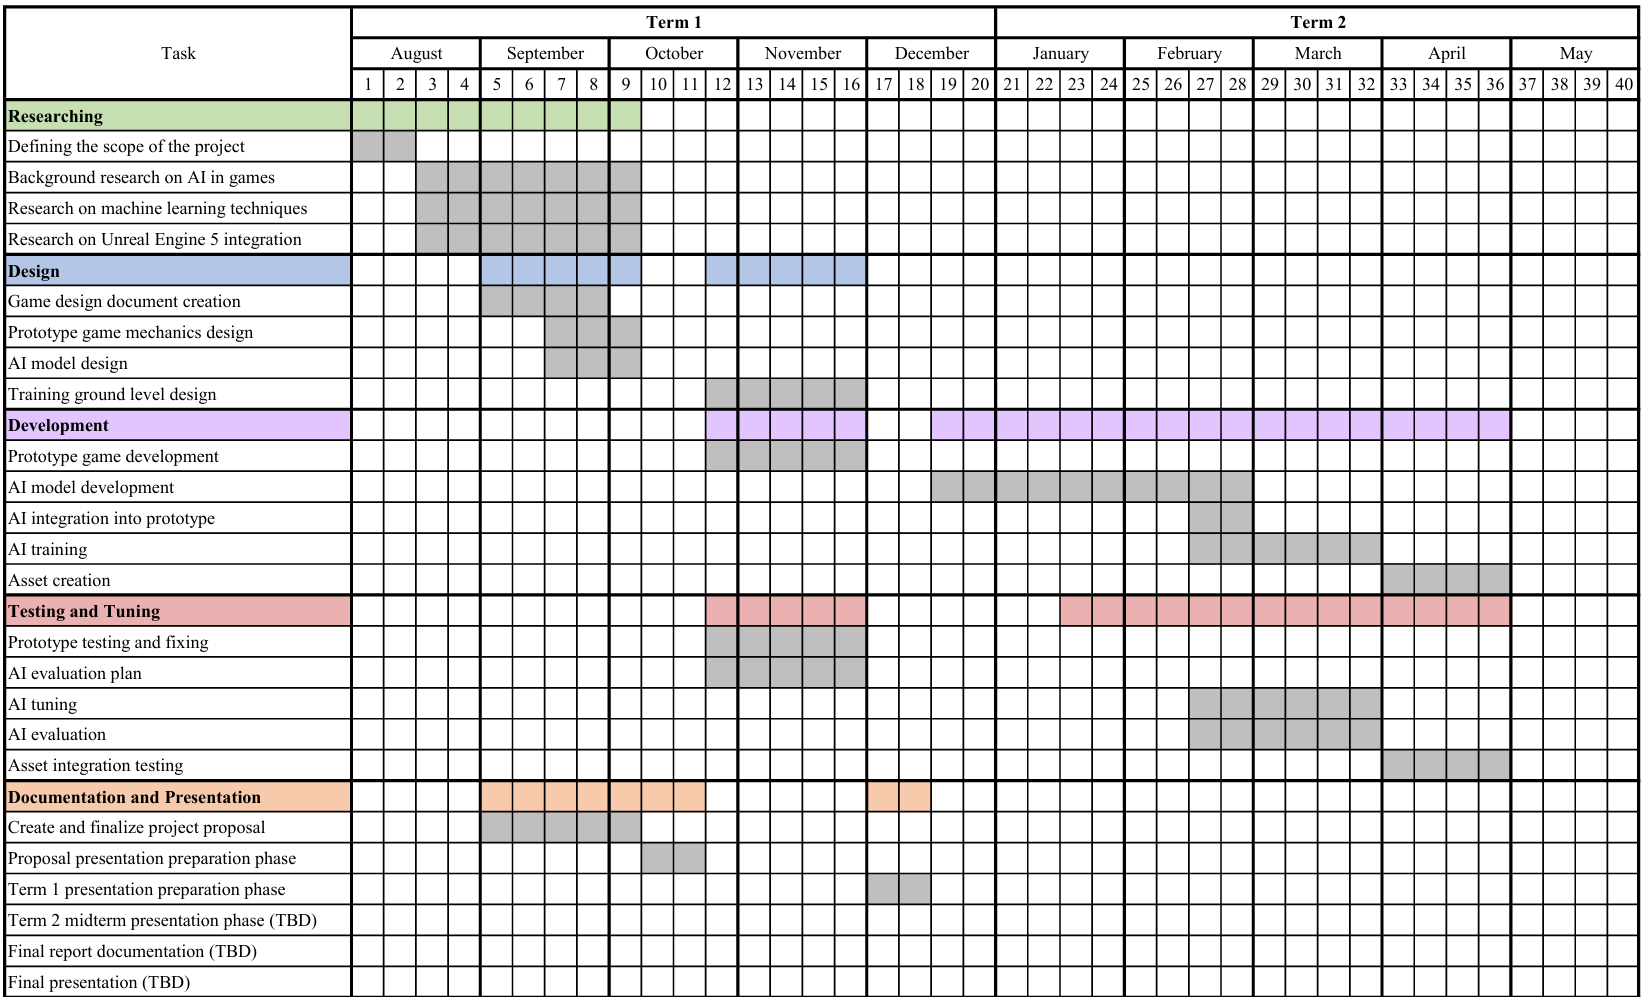
\includegraphics[width=15cm]{./Attachments/GanttChart.png}}
\caption{Gantt Chart}\label{fig:Gantt Chart}
\end{figure}
%%%%%%%%%%%%%%%%%%%%%%%%%%%%%%%%%%%%%%%%%%%%%%%%%%%%%%%%%%%%
%%%%%%%%%%%%%%  Literature Review %%%%%%%%%%%%%%%%%%%%%%%%%%
%%%%%%%%%%%%%%%%%%%%%%%%%%%%%%%%%%%%%%%%%%%%%%%%%%%%%%%%%%%%
\chapter{Background Theory and Related Work}
\section{Introduction}
This chapter provides the essential background knowledge and theoretical foundations necessary to understand the development of adaptive artificial intelligence (AI) in game environments. It covers key concepts, technologies, and programming languages utilized in AI development, with a focus on machine learning techniques such as reinforcement learning and relevant level design principles. Additionally, this chapter will explore related research and existing solutions, offering insights into the current state of AI in game development.

%This is how you add website url. -> \url{http://www.cpe.kmutt.ac.th}
%Explain theory, algorithms, protocols, or existing research works and tools related to your work.
%You can cite your references like this -> \cite{santi05b}  or multiplie cite like this -> \cite{bworld,hypersense}

\section{Theories and Core Concepts}
\subsection{Game Development}
\subsubsection{Game Development Life Cycle}
Game development is a complex and multifaceted process that involves various stages, from initial concept to the final product. The main stages include:
\begin{itemize}
\item  \textbf{Pre-production:} Conceptualization, storyboarding, and planning of the game. This stage defines the genre, mechanics, platform, and overall vision for the game.
\item  \textbf{Production:} The actual creation of the game, which includes coding, asset creation (art, sound, and animations), level design, and initial testing.
\item  \textbf{Post-production:} Refining the game through bug fixes, balancing, optimization, and quality assurance. This is also when the game is released to the public, followed by ongoing support such as updates and patches.
\end{itemize}
Throughout all stages, collaboration among developers, designers, artists, and sound engineers is essential to creating a cohesive experience. Game development today often involves teams of varying sizes, from small indie developers to large studios with hundreds of team members.
\subsubsection{Game Design}
Game design encompasses various elements that contribute to a game’s playability, engagement, and overall success:
\begin{itemize}
\item  \textbf{Game Mechanics:}
The rules and systems that govern how the game works. These include the physics, player controls, objectives, and win/lose conditions.
\item  \textbf{Story and Narrative:}
The storyline or plot that guides the player through the game. This can range from minimal or abstract narratives to fully immersive stories with complex characters and world-building.
\item  \textbf{Level Design:}
The creation of game environments and how players progress through them. Effective level design includes balancing challenge, pacing, and exploration, often introducing new elements at each stage to maintain player interest.
\item  \textbf{Assets:}
Game assets refer to the components used to build the visual, auditory, and interactive elements of a game. These include:
\begin{itemize}
\item  \textbf{Visual Assets:} Textures, 3D models, 2D sprites, animations, and visual effects that define the game's appearance.
\item  \textbf{Audio Assets:} Sound effects, background music, and character voices that create the auditory experience.
\item  \textbf{Code Assets:} Scripts and algorithms that govern game mechanics, AI behavior, and interactive elements.
\item  \textbf{UI Assets:} Icons, buttons, menus, and other user interface components.
\end{itemize}
Assets are the building blocks of any game, providing the necessary materials to bring concepts to life. Their quality and integration play a significant role in defining the overall aesthetic and functionality of the game.
\item  \textbf{User Interface (UI) and User Experience (UX):}
The design of menus, HUDs (heads-up displays), and the interaction flow. A clean and intuitive UI is critical for keeping players immersed in the game.
\end{itemize}
\subsubsection{Challenges Faced by Developers}
\begin{itemize}
\item  \textbf{Resource Limitations:}
Small teams often lack the budget and manpower to implement complex systems like advanced AI, detailed art, or high-end graphics
\item  \textbf{Complexity of Game Design:}
The more complex the game, the harder it is to manage. Creating a balanced and fun experience while ensuring that the game performs well across different platforms is a constant challenge.
\item  \textbf{Market Saturation:}
With the rise of digital storefronts and indie game platforms, the market is flooded with games, making it hard for any individual title to stand out.
\item  \textbf{Time Constraints:}
Many indie developers work on tight deadlines, often needing to finish a game within a limited period to avoid budget overruns or loss of momentum.
\end{itemize}
\subsubsection{The Increasing Demand for Adaptive and Dynamic Gameplay}
Players today expect more than static, predictable game experiences. They want games to react to their choices in real-time, creating a more dynamic and immersive experience. This demand has led to the integration of more advanced AI systems that can adapt and respond to player behavior in meaningful ways.\par
Games like \emph{The Witcher 3} and \emph{Horizon Zero Dawn} offer NPCs that respond realistically to the player’s actions, creating a sense of a living world. This trend toward dynamic and reactive gameplay is challenging for developers, especially smaller teams with limited resources, as it often requires implementing sophisticated AI and adaptive systems that can learn and evolve.

\subsection{Artificial Intelligence}
Artificial Intelligence (AI) in gaming refers to the simulation of human-like intelligence and decision-making processes in game entities. It plays a vital role in enhancing the interactivity and immersion of games by enabling non-player characters (NPCs) to exhibit responsive and believable behaviors. AI in games can range from simple rule-based systems to sophisticated machine learning models that adapt and evolve over time.
\subsubsection{Types of AI in Game Development}
\begin{itemize}
\item  \textbf{Finite State Machines (FSMs):}
FSMs are one of the simplest AI systems used in games. They consist of a finite set of states (e.g., idle, attack, flee) and predefined transitions between these states based on specific conditions. FSMs are easy to implement but may lead to predictable and repetitive behaviors.
\item  \textbf{Behavior Trees:}
Behavior trees are hierarchical structures used to manage decision-making processes. They allow for more modular and reusable AI behaviors compared to FSMs, making them popular in modern game development for controlling NPCs.
\item  \textbf{Utility-Based AI:}
This system evaluates different actions based on a utility score, selecting the action with the highest score. Utility-based AI allows NPCs to make decisions based on dynamic priorities, leading to more flexible and context-aware behaviors.
\item  \textbf{Pathfinding and Navigation:}
AI-controlled entities often need to move through complex environments. Pathfinding algorithms like A* (A-star) are widely used to calculate the shortest or most efficient paths, avoiding obstacles and optimizing movement.
\item  \textbf{Machine Learning in Games:}
Machine learning (ML) introduces adaptability and dynamic behaviors that traditional systems cannot achieve. Techniques like reinforcement learning enable AI agents to learn from their interactions with the environment, improving their performance over time. These systems can produce more realistic, challenging, and unpredictable NPCs.
\end{itemize}
\subsubsection{Applications of AI in Game Development}
\begin{itemize}
\item  \textbf{NPC Behavior and Opponent AI:}
AI is commonly used to control NPCs, making them act as enemies, allies, or neutral characters. The goal is to create behaviors that challenge and engage players without being overly predictable or frustrating.
\item  \textbf{Procedural Content Generation (PCG):}
AI can generate game assets such as levels, characters, and items dynamically. This enhances replayability and reduces development time by automating repetitive tasks.
\item  \textbf{Game Testing and QA:}
Adaptive AI agents can be trained to simulate player behaviors, identifying bugs, balancing gameplay, and stress-testing game mechanics during development.
\item  \textbf{Player Profiling and Personalization}
AI systems can analyze player data to adapt the gameplay experience, tailoring difficulty, content, and narratives to individual player preferences.
\end{itemize}
\subsubsection{Advantages of AI in Game Development}
\begin{itemize}
\item  \textbf{Dynamic and Immersive Gameplay:}
Adaptive AI creates experiences that feel more responsive and personalized.
\item  \textbf{Enhanced Development Efficiency:}
Automating tasks like testing, content generation, and debugging reduces time and costs.
\item  \textbf{Scalability:}
AI systems can be designed to adapt across different game genres and mechanics, enabling reusable assets.s
\end{itemize}
\subsubsection{Challenges of AI in Game Development}
\begin{itemize}
\item  \textbf{Development Costs:}
Advanced AI systems require significant computational resources and expertise, which can be a challenge for indie developers.
\item  \textbf{Complexity in Balancing:}
Creating an AI that is both challenging and fair to players requires careful design and testing.
\item  \textbf{Unpredictable Outcomes:}
In adaptive systems, emergent behaviors may lead to unintended gameplay consequences.
\end{itemize}
AI in game development is an ever-evolving field, driven by advances in computational power and machine learning algorithms. It holds tremendous potential for creating smarter, more immersive games while addressing development bottlenecks like scalability and automation.

\subsection{Machine Learning}

Machine learning involves programming computers to optimize a performance criterion based on example data or past experiences. It entails constructing models capable of recognizing patterns or regularities in data, enabling systems to make predictions, adapt, or gain insights. Grounded in statistical theory, machine learning employs efficient algorithms to manage large datasets and perform complex computations. It has widespread applications in fields such as retail, finance, healthcare, and telecommunications, addressing challenges like prediction, optimization, and pattern recognition.\par

Machine learning algorithms are commonly categorized into three types based on their learning paradigm: supervised learning, unsupervised learning, and reinforcement learning.

\subsubsection{Supervised Learning}
Supervised learning relies on labeled datasets, where the correct outcome is predefined, to train models. These models predict outcomes based on input data and refine predictions by learning from errors. Supervised learning is frequently applied in classification and regression tasks.
\begin{itemize}
\item  \textbf{Naive Bayes:} Naive Bayes is a classification method based on Bayes Theorem, assuming that features are independent of each other. There are three types: Multinomial, Bernoulli, and Gaussian Naive Bayes. It's commonly used in text classification, spam detection, and recommendation systems.
\item  \textbf{K-nearest neighbor:} KNN is a non-parametric algorithm that classifies data points based on proximity, usually using Euclidean distance. It’s simple and efficient for small datasets but becomes slower as the dataset grows. KNN is often used in recommendation engines and image recognition.
\item  \textbf{Random forest:} Random forest is a flexible supervised algorithm for classification and regression, combining multiple decision trees to reduce variance and improve accuracy.
\end{itemize}

\subsubsection{Unsupervised Learning}
Unsupervised learning models analyze unlabeled data to discover hidden patterns or structures. This approach is typically applied in clustering, dimensionality reduction, and anomaly detection.
\begin{itemize}
\item  \textbf{K-means clustering:} K-means clustering groups data points into K clusters based on their distance from the centroids. Larger K values create smaller, more granular groups, while smaller K values result in larger clusters. It's widely used in market segmentation, document clustering, and image compression.
\item  \textbf{Principal component analysis (PCA):} PCA is a dimensionality reduction method that transforms data into new components, maximizing variance while reducing redundancy. Each successive component is uncorrelated and orthogonal to the previous one, capturing the most variance in fewer dimensions.
\item  \textbf{Autoencoders:} Autoencoders use neural networks to compress and reconstruct data, with the hidden layer acting as a bottleneck. The process is split into \emph{encoding} (input to hidden layer) and \emph{decoding} (hidden layer to output).
\end{itemize}

\subsubsection{Reinforcement Learning}
Reinforcement learning allows an agent to learn by interacting with an environment to achieve a specific goal. Mimicking trial-and-error learning, RL optimizes actions using rewards for goal-oriented behaviors and penalties for undesirable actions. This iterative process helps the agent refine its strategy to maximize cumulative rewards.

Key Components of RL:
\begin{itemize}
\item  \textbf{Agent:} The learner or decision-maker.
\item  \textbf{Environment:} The system with which the agent interacts.
\item  \textbf{Actions:} Choices available to the agent.
\item  \textbf{Rewards:} Feedback to guide the agent's learning process.
\item  \textbf{Policy:} The strategy determining the agent's actions.
\end{itemize}
\begin{figure}[!h]
\centering
\fbox{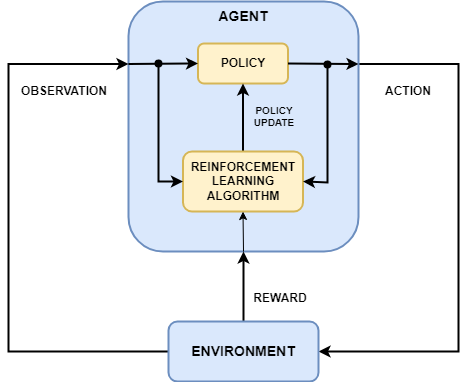
\includegraphics[width=10cm]{./Attachments/ReinforceModelDia.png}}
\caption{Reinforce Learning Model Diagram}\label{fig:ReinforceModelDia}
Source:
\href{https://www.mathworks.com/help/reinforcement-learning/ug/what-is-reinforcement-learning.html} {https://www.mathworks.com/help/reinforcement-learning/ug/what-is-reinforcement-learning.html}
\end{figure}
In game development, RL is particularly useful for training adaptive AI that can learn and evolve based on player interactions. This enables the creation of NPCs with more dynamic and challenging behaviors, as well as automated game testing agents that evaluate game mechanics and balance.
\subsection{Reinforcement Learning}
Reinforcement learning (RL) focuses on training agents to make sequences of decisions by interacting with an environment. The agent learns to optimize a long-term reward by observing states, taking actions, and receiving feedback in the form of rewards or penalties. This section explores key RL algorithms relevant to game development and their applications.
\subsubsection{Q-Learning}
Q-Learning is one of the simplest RL algorithms that builds a Q-value table to represent the expected future rewards for every state-action pair.\par
\textbf{Mathematical Foundation} \\
The Bellman Equation updates the Q-value for a given state-action pair iteratively
\begin{equation}
Q(s, a) \gets Q(s, a) + \alpha(r + \gamma max_{a}(Q(s', a')) - Q(s, a))
\end{equation}
\begin{itemize}
\item $Q(s,a)$: Current Q-value for state $s$ and action $a$.
\item $s$: Current state
\item $a$: Current action
\item $r$: Reward received after taking action $a$ in state $s$
\item $a'$: Next action
\item $s'$: Next state
\item $\alpha$: Learning rate, controlling the size of the update step.
\item $\gamma$: Discount factor, determining the importance of future rewards.
\end{itemize}
\textbf{Key Features}
\begin{itemize}
\item Off-policy: It learns the optimal policy independently of the agent’s actions.
\item Suitable for discrete and small state-action spaces.
\end{itemize}
\textbf{Use Case in Games} \\
Training AI for grid-based games like Snake or Pac-Man.\par
\textbf{Psuedocode}
\begin{algorithm}
\caption{Q-Learning Algorithm}\label{alg:QLA}
\begin{algorithmic}
\State Initialize Q-table with zeros
\For{\texttt{each episode}}
\State Initialize state s
\While{\texttt{not done}}
	\State Choose action a using epsilon-greedy policy
	\State Take action $a$, observe reward $r$ and next state $s'$	
	\State  Update Q-value:
	\State  $Q(s, a) \gets Q(s, a) + \alpha * (r + \gamma * max(Q(s', a')) - Q(s, a))$
	\State $s = s'$
\EndWhile
\EndFor
\end{algorithmic}
\end{algorithm}
\subsubsection{Deep Q-Learning (DQN)}
DQN scales Q-Learning to environments with continuous or high-dimensional state spaces by approximating the Q-function using a deep neural network.\par
\textbf{Enhancements over Q-Learning:}
\begin{itemize}
\item  \textbf{Experience Replay:} Stores past transitions $(s,a,r,s')$ in a replay buffer, sampling mini-batches for training to reduce correlation.
\item  \textbf{Target Network:}  A separate network for computing target Q-values, updated less frequently to stabilize training.
\end{itemize}
\textbf{Key Equations} \\
Update the neural network weights $\theta$ by minimizing the loss:
\begin{equation}
L(\theta) = 	\mathbb{E}_{(s,a,r,s')}[(r + \gamma max_{a}Q(s',a;\theta^-)-Q(s,a;\theta))^2]
\end{equation}
\begin{itemize}
\item $L(\theta)$: The loss function, a measure of how far the model's predictions are from the true or desired values.
\item $Q(s,a;\theta)$: $Q(s,a)$ approximate using neural network $\theta$.
\item $\theta$: Parameters of a neural network used to approximate a function.
\item $\mathbb{E}$: The average value of the loss across sampled data points.
\end{itemize}
\textbf{Use Case in Games} \\
Training agents in platformers, complex strategy games, or visual navigation tasks.\par
\textbf{Psuedocode}
\begin{algorithm}
\caption{Deep Q-Learning Algorithm}\label{alg:DQLA}
\begin{algorithmic}
\State Initialize replay buffer and Q-network
\For{\texttt{each episode}}
\State Initialize state s
\While{\texttt{not done}}
	\State Choose action a using epsilon-greedy policy
	\State Take action $a$, observe reward $r$ and next state $s'$	
	\State Store transition (s, a, r, s') in replay buffer
	\State Sample mini-batch from replay buffer
	\State Compute target: $y = r + \gamma max(Q_target(s', a'))$
	\State Update Q-network using gradient descent
	\State Periodically update target network
\EndWhile
\EndFor
\end{algorithmic}
\end{algorithm}
\subsubsection{Policy Gradient Methods}
Policy gradient methods optimize the policy directly by maximizing the expected reward.\par
\textbf{Policy Representation} \\
The policy is parameterized as $\pi_{\theta}(a|s)$, where $\theta$ are the weights of the model. \\
\textbf{Objective Function}
\begin{equation}
J(\theta) = \mathbb{E}_{\pi_{\theta}}[\sum_{t} \gamma^{t}r_{t}]
\end{equation}
\textbf{Gradient Update:} \\
Using the policy gradient theorem:
\begin{equation}
\nabla_{\theta}J(\theta) = \mathbb{E}[\nabla_{\theta}log\pi_{\theta}(a|s)R]
\end{equation}
where $R$ is the cumulative reward.\par
\textbf{Use Case in Games} \\
Training agents in games requiring smooth control, such as racing or flight simulators.\par
\textbf{Psuedocode}
\begin{algorithm}
\caption{Policy Gradient Methods}\label{alg:PGM}
\begin{algorithmic}
\State Initialize policy network
\For{\texttt{each episode}}
\State Collect trajectory of states, actions, and rewards
\State Compute discounted rewards for each state
\State Update policy network to maximize log-probability of actions weighted by rewards
\EndFor
\end{algorithmic}
\end{algorithm}
\subsubsection{Proximal Policy Optimization (PPO)}
PPO improves policy gradient methods by introducing a clipped objective to ensure stable updates.\par
\textbf{Objective Function}
\begin{equation}
L^{CLIP}(\theta) = \mathbb{E}[\min(r_{t}(\theta)A_{t}, clip(r_{t}(\theta), 1 - \epsilon, 1 + \epsilon)A_{t}]
\end{equation}
where $r_{t}(\theta)$ is the probability ratio, $A_{t}$ is the advantage estimate, and $\epsilon$ is a hyperparameter for clipping.\par
\textbf{Key Features}
\begin{itemize}
\item Prevents large policy updates.
\item Balances performance and training stability.
\end{itemize}
\textbf{Use Case in Games} \\
Robust AI for large-scale multi-agent systems or highly variable environments.\par
\textbf{Psuedocode}
\begin{algorithm}
\caption{Proximal Policy Optimization}\label{alg:PPO}
\begin{algorithmic}
\For{\texttt{each iteration}}
\State Collect trajectories using current policy
\State Compute advantages using value function
\State Update policy network using clipped surrogate objective
\State Update value network to reduce value estimation error
\EndFor
\end{algorithmic}
\end{algorithm}
\subsubsection{Actor-Critic Methods}
Actor-Critic combines policy optimization (actor) with value function estimation (critic).\par
\textbf{Advantages} 
\begin{itemize}
\item Prevents large policy updates.
\item Balances performance and training stability.
\end{itemize}
\textbf{Variants}
\begin{itemize}
\item  \textbf{A2C:} Uses synchronous updates with multiple workers.
\item  \textbf{A3C:} Parallelizes training by running multiple agents asynchronously.
\end{itemize}
\textbf{Use Case in Games} \\
Real-time strategy games requiring fast adaptation.\par
\textbf{Psuedocode}
\begin{algorithm}
\caption{Actor-Critic Methods}\label{alg:ACM}
\begin{algorithmic}
\For{\texttt{each iteration}}
\State Collect trajectories from actor network
\State Compute value targets using critic network
\State Update actor to maximize policy objective
\State Update critic to minimize value estimation error
\EndFor
\end{algorithmic}
\end{algorithm}
\subsubsection{Multi-Agent Reinforcement Learning (MARL)}
In MARL, multiple agents learn and interact in a shared environment, adapting strategies collaboratively or competitively.\par
\textbf{Key Challenges} 
\begin{itemize}
\item Coordination among agents.
\item Balancing exploration and exploitation in dynamic environments.
\end{itemize}
\textbf{Applications in Games}
\begin{itemize}
\item Multiplayer strategy games.
\item Cooperative tasks in simulation-based training.
\end{itemize}

\begin{table}[H]
\caption{Comparison of RL Algorithms}\label{tbl:ComparisonofRLAlgorithms}
\renewcommand{\arraystretch}{1.5} % Increase row height
\setlength{\tabcolsep}{4pt} % Adjust column padding
\begin{tabularx}{\textwidth}{|>{\raggedright\arraybackslash}X|>{\raggedright\arraybackslash}X|>{\raggedright\arraybackslash}X|>{\raggedright\arraybackslash}X|}
\hline
\textbf{Algorithm} & \textbf{Advantages} & \textbf{Limitations} & \textbf{Suitable Games} \\ \hline
\textbf{Q-Learning} & Simple, effective for small problems. & Struggles with large state spaces. & Grid-based games, Puzzles \\ \hline
\textbf{Deep Q-Learning (DQN)} & Handles complex state spaces. & Computationally intensive. & Platformers, Visual games \\ \hline
\textbf{Policy Gradient} & Works well in continuous action spaces. & Susceptible to instability. & Racing, Flight simulators \\ \hline
\textbf{PPO} & Stable, efficient in diverse scenarios. & Trade-off between stability and speed. & Scalable multi-agent games \\ \hline
\textbf{Actor-Critic} & Fast convergence, suitable for real-time games. & Requires careful tuning. & Real-time strategy games, Simulators \\ \hline
\textbf{MARL} & Enables collaborative/competitive AI. & Complexity increases with agent count. & Multiplayer games, Co-op challenges \\ \hline
\end{tabularx}
\end{table}

\section{Development Tools}

\subsection{Unity}
Unity is a versatile and widely-used game development engine renowned for its ease of use, flexibility, and strong support for both 2D and 3D projects. It was chosen for this project due to its compatibility with machine learning tools, efficient workflow, and robust asset pipeline. Unity provides a range of tools for AI development, including the Unity ML-Agents Toolkit, NavMesh systems, and animation controllers, which enable the creation of intelligent and adaptive behaviors. These tools allow AI agents to interact with their environment, learn from rewards, and optimize performance effectively.

%\begin{figure}[!h]
%\centering
%\fbox{
\includegraphics[width=10cm]{./Attachments/UnityLogo.png}}
%\caption{Unity Logo}\label{fig:UnityLogo}
%\end{figure}

\begin{itemize}
\item  \textbf{ML-Agents Capabilities}
Unity’s ML-Agents Toolkit is a robust feature for integrating machine learning into game development. It supports training AI agents using techniques like reinforcement learning (RL), imitation learning, and other advanced approaches. Key features include:
\begin{itemize}
\item  \textbf{Reinforcement Learning:} ML-Agents supports deep reinforcement learning (DRL), enabling agents to learn through interactions with the environment by maximizing cumulative rewards. This is particularly suitable for developing adaptive AI behaviors in platformer games.
\item  \textbf{Training Environments:} It simplifies the creation of training environments, allowing agents to interact with dynamic game worlds, respond to stimuli (e.g., obstacles or goals), and improve their performance iteratively.
\item  \textbf{Training with Multiple Agents:} The toolkit supports simultaneous training of multiple agents in the same environment, ideal for creating coordinated enemy behaviors or competitive agents.
\item  \textbf{Sensor Integration:} ML-Agents accommodates various sensors (e.g., visual, ray-casting, and custom inputs), enabling agents to gather feedback from the game world for informed decision-making.
\item  \textbf{Model Export:} Trained models can be exported in the ONNX (Open Neural Network Exchange) format for seamless deployment in Unity, integrating advanced AI behavior into gameplay.
\end{itemize}
\item  \textbf{2D Game Support:}
Unity's native 2D tools, including Tilemaps, physics, and animation systems, streamline the creation of platformer environments. This aligns perfectly with the project's goals by facilitating a smooth workflow for designing levels and mechanics.
\end{itemize}

\subsection{C\#}
C\# is Unity's primary programming language, offering an optimal balance of performance, ease of use, and flexibility. It is instrumental in implementing game mechanics and AI behaviors.
\begin{itemize}
\item  \textbf{Performance Optimization:} C\# enables efficient scripting for real-time calculations, game events, and AI logic. Its clean syntax and extensive libraries ensure that resource-intensive tasks, such as agent movement and obstacle detection, run efficiently.
\item  \textbf{Custom Gameplay Features:} Using C\#, developers can create custom gameplay mechanics, such as pathfinding, player interactions, and dynamic environmental elements. Unity's scripting API provides precise control over agents and game objects, offering flexibility that extends beyond built-in tools.
\end{itemize}

\subsection{Python}
Python is a widely-used programming language in machine learning and AI development, known for its simplicity, flexibility, and extensive ecosystem of libraries. In this project, Python plays a critical role in developing and training AI models.
\begin{itemize}
\item  \textbf{Machine Learning Development:} Python, in combination with PyTorch, is used to implement reinforcement learning algorithms (e.g., Deep Q-Networks, Proximal Policy Optimization) for training AI agents. Its high-level syntax accelerates experimentation and prototyping, making it ideal for AI development.
\item  \textbf{Data Processing:} Libraries like NumPy and Pandas are used for pre-processing and analyzing training data, enabling efficient monitoring of agent performance and model behavior.
\item  \textbf{Integration with Unity:} 
Trained models developed in Python can be exported (e.g., using ONNX) and integrated into Unity, where they control agent behavior within the game environment.
\end{itemize}

\subsection{PyTorch}
PyTorch is an open-source machine learning library widely used for deep learning and reinforcement learning. It plays a crucial role in this project for developing, training, and fine-tuning AI models to operate within the Unity environment.
\begin{itemize}
\item  \textbf{Reinforcement Learning Compatibility:}
PyTorch supports key reinforcement learning algorithms such as Deep Q-Networks (DQN) and Proximal Policy Optimization (PPO). These algorithms are integral to training AI agents, enabling them to interact with and learn from the game environment by adapting strategies based on feedback and rewards.
\item  \textbf{GPU Acceleration:}
PyTorch’s GPU acceleration significantly reduces training time for neural networks. This allows for faster iteration and experimentation, facilitating efficient model development and parameter tuning.
\item  \textbf{Integration with Unity:}
Although PyTorch is Python-based, trained models can be exported in ONNX or other compatible formats for integration into Unity. This ensures that machine learning models seamlessly control in-game agents during gameplay, bridging the gap between AI development and deployment.
\end{itemize}

\subsection{GitHub}
GitHub is a version control and collaboration platform that facilitates the management of source code and assets throughout the project's development.
\begin{itemize}
\item  \textbf{Version Control:}
GitHub enables efficient version tracking, allowing developers to monitor changes to the codebase and revert to previous versions when necessary. This ensures stability and helps maintain control over the evolving project.
\item  \textbf{Collaboration:}
GitHub supports team collaboration by allowing multiple developers to work simultaneously on different parts of the project. The platform's branching and pull request features ensure an organized and efficient development workflow, enabling seamless merging of contributions.
\item  \textbf{Backup and Deployment:} 
The repository serves as a secure backup for all project files and assets. Additionally, GitHub Actions can automate tasks such as deployment and testing, streamlining development and ensuring smooth continuous integration.
\end{itemize}

\section{Related research}

\subsection{Automated Playtesting in Game Development}
Playtesting is an important part of game development since it ensures that the challenges are balanced, systems work properly, and the player experience remains enjoyable. Traditionally, this process has relied on manual testers, which may be time-consuming and costly. In response to these issues, Sriram (2019) researches the use of deep reinforcement learning (DRL) and curriculum learning to automate playtesting in 2D platformer games. His research introduces an Automated Playtesting (APT) program that trains AI agents to explore game levels, discovering design defects and gameplay imbalances without the need for operator input. By gradually increasing level complexity, these AI agents learn to adapt and manage a wide range of in-game events, making them useful for assessing new levels.\par
\begin{figure}[!h]
\centering
\fbox{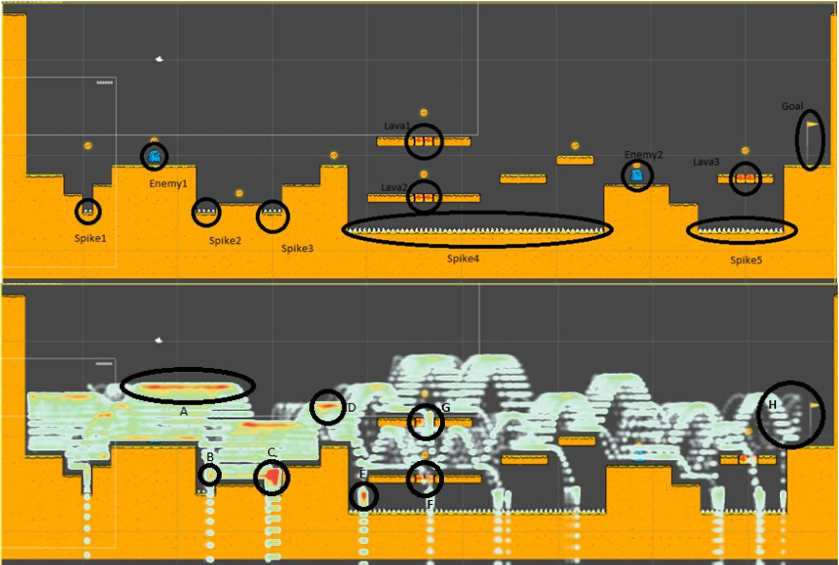
\includegraphics[width=10cm]{./Attachments/Automatebugtest.png}}
\caption{Unseen level and Unseen level with the agent heat map}\label{fig:UnseenLevel}
Source:
\href{https://repository.library.northeastern.edu/files/neu:m0455c95d/fulltext.pdf}{https://repository.library.northeastern.edu/files/neu:m0455c95d/fulltext.pdf} 
\end{figure}
Sriram's methodology provides a data-driven strategy for playtesting, but it is not the only option. Scripted AI agents are a more traditional approach, as they follow specific rules and behaviors rather than learning flexibly. These bots are easier to implement and use far less computational resources. However, they lack flexibility, which means they cannot generalize well across game levels or detect unexpected gameplay problems. In comparison, DRL-based playtesting is a versatile and scalable method that is especially helpful for games with automated generation or advanced level designs.\par
\newpage
\subsection{AI Techniques in 2D Platformer Games}
AI is an important tool for creating interesting yet challenging gameplay, particularly in platform games. In this area, AI behavior greatly influences player interest and difficulty. To improve AI behavior, Persson (2005) studies three AI methods: pathfinding, image recognition, and line of sight. Their research focuses on AI movement and perception for more realistic interactions. The detection of line of sight ensures that the opponents will never see the player unless there are no obstacles in their path, preventing their irrational behavior. If they see changes in their environment with the aid of image recognition, then the AI will make appropriate changes to their actions. Finally, pathfinding algorithms enable AI to traverse complex levels, allowing for accurate movement while following or avoiding players.\par
\begin{figure}[!h]
\centering
\fbox{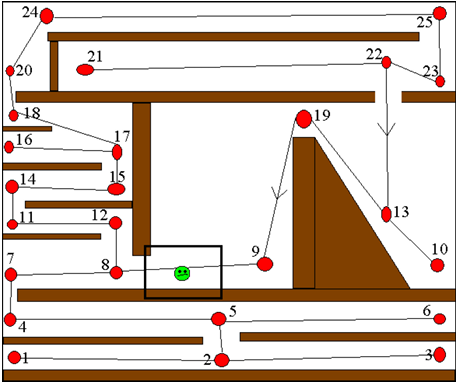
\includegraphics[width=10cm]{./Attachments/AITechniquesin2DPlatformerGames.png}}
\caption{In a 2D platform game, pathfinding nodes are shown as ellipse with corresponding indexes and connections on the map.}\label{fig:AITechniq}
Source:
\href{https://www.diva-portal.org/smash/get/diva2\%3A4762/FULLTEXT01.pdf?utm\_source=chatgpt.com}{https://www.diva-portal.org/smash/get/diva2\%3A4762/FULLTEXT01.pdf?utm\_source=chatgpt.com}
\end{figure}
Behavior trees and FSMs make for an alternative pseudo-scientific contrast, they would be a fit in the context of game AI. FSMs provide a fixed, predictable AI behavior strategy, tending to have an extraordinarily rigid structure that requires much tuning to reproduce complex interactions. Behavior trees are about modularity and scalability, but still, they lack dynamically generated structures for decision making. Persson's solution offers a system that is more dynamic in character than pure FSM-based behavior systems but suffers from a downslope in computation.\par
\newpage
\subsection{Pathfinding and Navigation in Platformer AI}
One main issue within platformer AI is making an intelligent movement deemed natural and responsive. Smith (2021) has proposed a physics-based pathfinding system that moves AI-controlled characters with a real-life dynamic principle for level navigation. The construction of a platform graph is established, with surfaces as nodes and possible movement trajectories as edges. AI agents use the A* pathfinding algorithm to determine optimal routes between platforms following the physics enforced by the game. This is not pure AI control since Smith's system translates movement decisions into simulated player inputs to guard against jerkiness and make motions feel natural.\par
\begin{figure}[!h]
\centering
\fbox{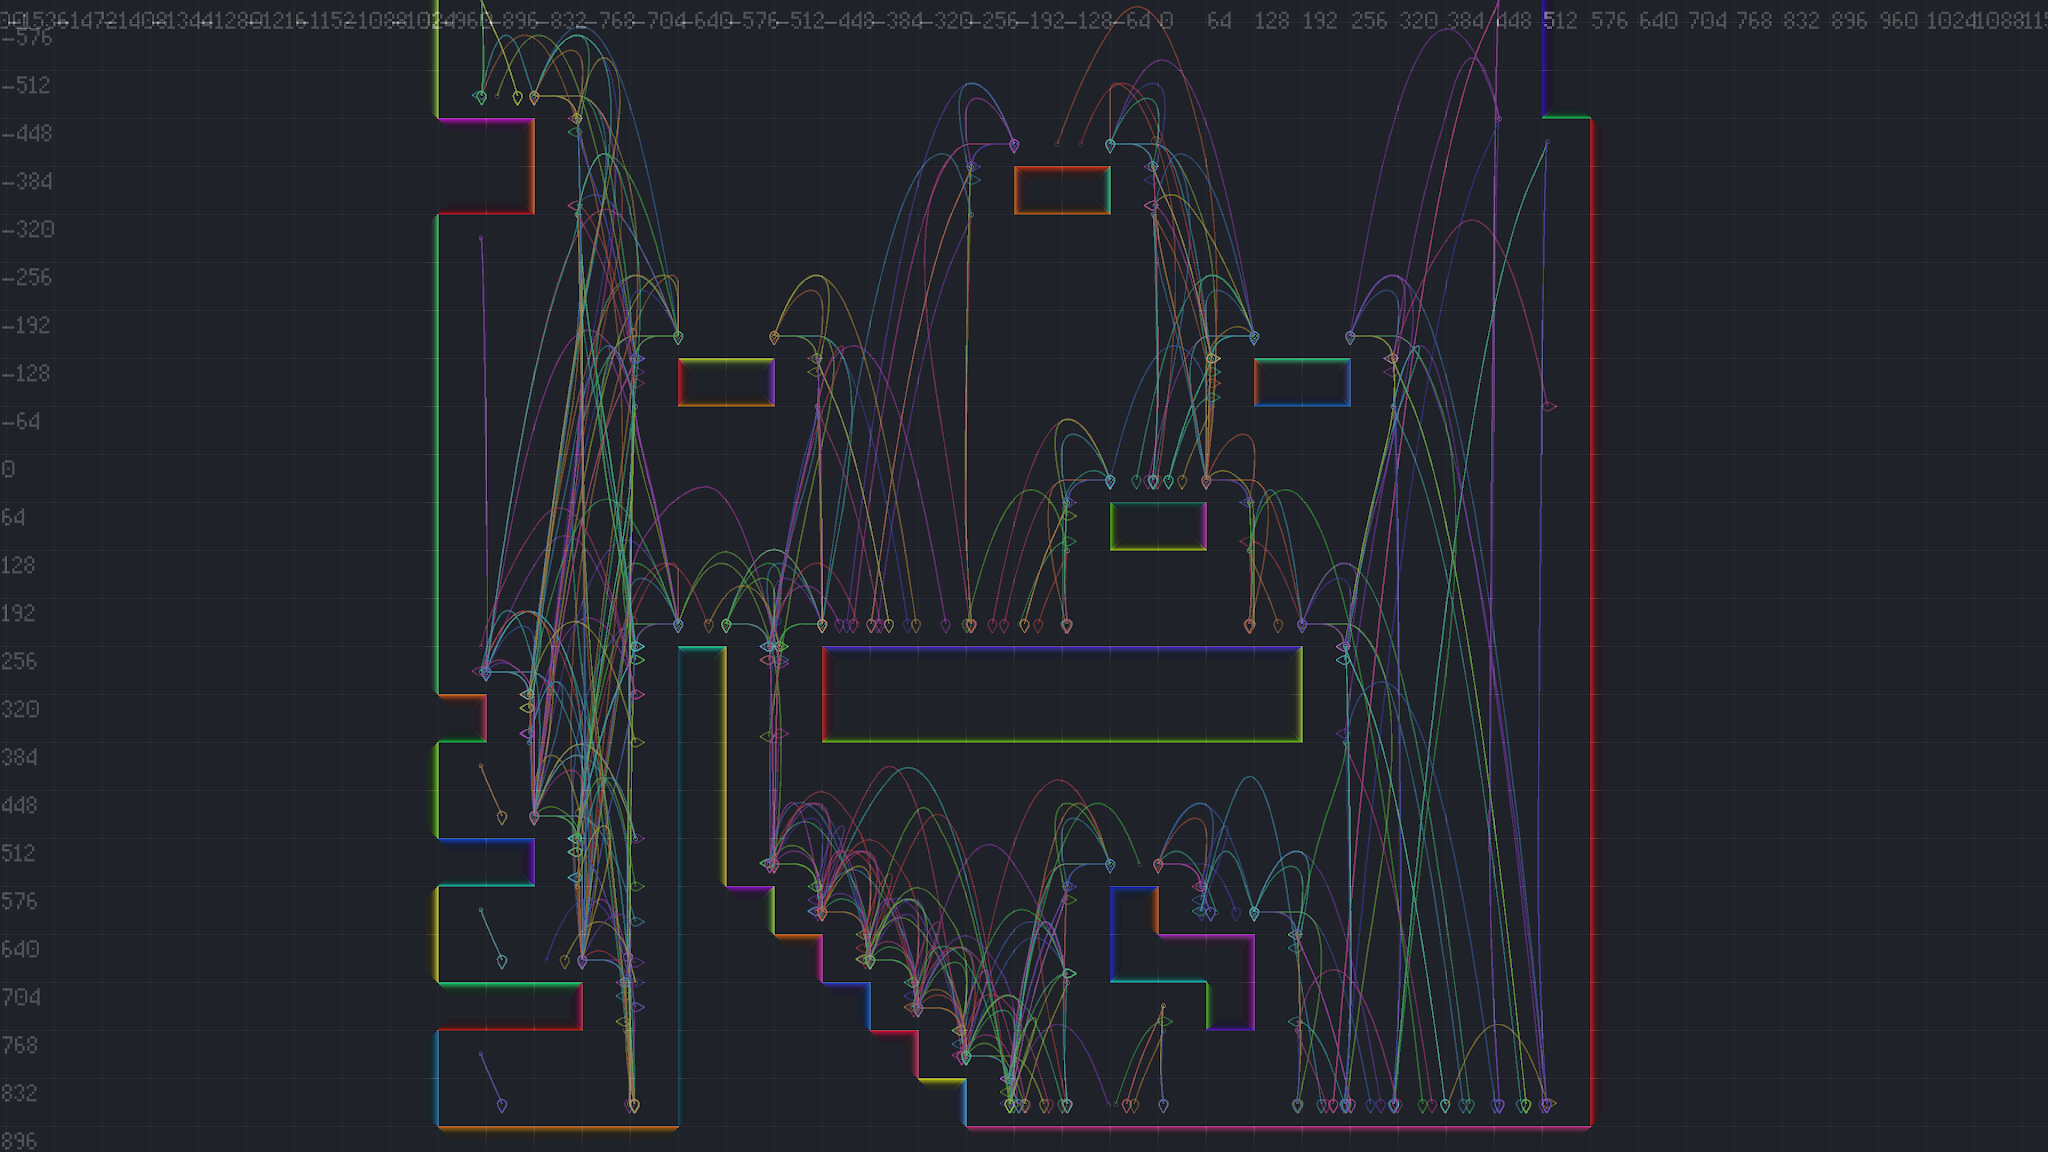
\includegraphics[width=10cm]{./Attachments/PathfindingandNavigationinPlatformerAI.png}}
\caption{Using A* search to find path through the graph}\label{fig:A*tofindPath}
Source:
\href{https://devlog.levi.dev/2021/09/building-platformer-ai-from-low-level.html?utm\_source=chatgpt.com}{https://devlog.levi.dev/2021/09/building-platformer-ai-from-low-level.html?utm\_source=chatgpt.com}  
\end{figure}
Smith's algorithmic approach, in contrast to machine learning-based navigation systems, allows for a greater degree of control and responsiveness. However, it is still limited. Deep reinforcement learning (DRL) would be an alternative approach to AI navigation, where agents would learn movement strategies through trial and error. On the one hand, the advantage of DRL-based AI is its adaptation to a dynamically changing environment; this, of course, comes alongside their requirement of extensive training and computation resources. Smith's method, conversely, is fast and reliable during runtime, for their physics-based paths are pre-calculated, yet they lack the adaptability of AI solutions based on DRL to tackle the unforeseen changes of levels.\par
\newpage
\section{Gap Analysis}
While there has been development in the area of AI-driven gameplay agents, there are still many fields with which one must dare to be precise. One, albeit a major limitation, is the fact that much study has been undertaken with very specific tasks or under very specific game environments, limiting the ability of agents to generalize through new levels or by game mechanics. Second, very few works consider the train environment in which both the player-like AIs and the opponent AIs coexist, thus foregoing any possible adversarial learning or mutual adaptation. Third, most prior work overlooks modularity or reusability, which are necessary for real applications in indie game development.\par

On the other hand, Mario AI-type benchmarks serve a useful purpose by defining a controlled experiment; however, they often do not cover the broader spectrum of challenges present in more complex or custom-built platformers. Thus, the need exists for flexible, open-ended environments where AI agents could be trained to interact with not just static platforms but also dynamic obstacles, NPCs, and contextual goals.\par
\section{How our work differs}
The project is different even from the past research in several key aspects. First, we have introduced a custom-designed 2D platformer environment specifically intended to aid in the training and testing of AI agents under different scenarios. Unlike previous benchmarks, our environment is modular and extendable, so new mechanics, enemies, and layout difficulties can really be added quickly.\par

Second, and importantly, this work trains and tests both types of agents at the same time: player agents and enemy agents. Since this dual-agent arrangement, it tends to make for more interesting and, hence, dynamic gameplay interaction scenarios, both in adversarial reinforcement learning settings where agents must adjust not only to their evolving environment but also to each other's evolving strategies.\par

Third, the AI models learned in this paper work are reusable and adaptable assets. By emphasizing modularity and generalization, we expect to provide tools usable across multiple games with minimal effort, thereby helping to fill a big hole in game AI software development-land, especially for those indie developers that operate on a shoestring budget.\par

Lastly, for this research, we apply Proximal Policy Optimization (PPO), a powerful and stable reinforcement learning algorithm that trains agents to adapt to complex platformer environments. This underscores our commitment to using scalable, state-of-the-art methodologies in real-time game AI.\par


% Can define this in the preamble..
%You can place the figure and refer to it as Figure~\ref{fig:model2}.
%The figure and table numbering will be run and updated automatically when you add/remove tables/figures from the document.

%\begin{figure}[!h]\centering
%\setlength{\fboxrule}{0.2mm} % can define this in the preamble
%\setlength{\fboxsep}{1cm}
%\fbox{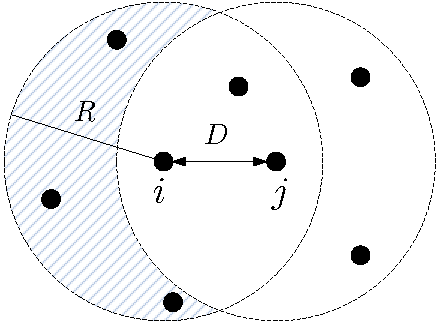
\includegraphics[width=5cm]{./model2.pdf}}
%\caption{The network model}\label{fig:model2}
%\end{figure}

%%%%%%%%%%%%%%%%%%%%%%%%%%%%%%%%%%%%%%%%%%%%%%%%%%%%%55
%%%%%%%%%%%%%%%%%%%%%%%%%%%%%%%%%%%%%%%%%%%%%%%%%%%%%
%%%%%%%%%%%%%%%%%%%%%%%%%%%%%%%%%%%%%%%%%%%%%%%%%%%%%
\chapter{METHODOLOGY AND DESIGN}

\section{Introduction}

This chapter outlines the methodology and design principles employed in the development of an adaptive artificial intelligence (AI) system tailored for 2D platformer games. The project integrates reinforcement learning into a modular AI framework, aiming to provide a reusable and easily extendable solution for game developers.\par

Building on the theoretical foundations established in the previous chapter, this section focuses on the practical aspects of system implementation. The goal is to bridge academic research in reinforcement learning with real-world game development tools and workflows. To achieve this, a structured, modular design was adopted to ensure flexibility, reusability, and compatibility across different 2D platformer projects.\par

This chapter will outline the key components of our methodology, including:
\begin{itemize}
\item \textbf{System Architecture:} An overview of the core system components, including Unity, ML-Agents, and the communication pipeline between the training environment and learning algorithm.
\item \textbf{Game Environment Design:} A description of the custom 2D platformer environment developed for training and evaluating AI behavior.
\item \textbf{AI Algorithms and Models:} The selection and implementation of reinforcement learning techniques, specifically Proximal Policy Optimization (PPO).
\item \textbf{Training Process and Optimization:} Details on training configuration, reward structure, curriculum learning considerations, and agent evaluation metrics.
\item \textbf{AI Integration and Packaging:} The process of embedding the trained AI into a Unity-compatible asset and enabling modular extensibility through custom action modules.
\end{itemize}

By following this methodology, the project aims to deliver a robust AI development framework that not only supports player and enemy agent training but also provides an accessible entry point for indie developers to integrate, extend, and retrain AI agents for their own games.\par
%Explain the design (how you plan to implement your work) of your project. Adjust the section titles below to suit the types of your work. Detailed physical design like circuits and source codes should be placed in the appendix.

\section{System Architecture}

The system architecture of this project is designed to support the development, training, and deployment of an adaptive artificial intelligence (AI) system within a Unity-based 2D platformer game. The architecture integrates multiple interconnected components, enabling seamless communication between Unity and external machine learning frameworks. These components include the training environment, agent behaviors, environment parameters, and the communication interface with the Python-based reinforcement learning trainer. Figure \ref{fig:SystemDiagram} illustrates the relationships between these components.\par

\begin{figure}[!h]
\centering
\fbox{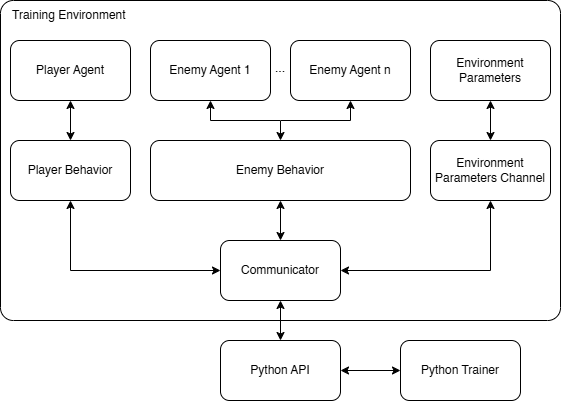
\includegraphics[width=10cm]{./Attachments/SystemDiagram.png}}
\caption{System Architecture Diagram, drawn on draw.io}\label{fig:SystemDiagram}
\end{figure}
\FloatBarrier
\subsection{Training Environment}
The training environment is a controlled simulation where AI agents interact, learn, and refine their decision-making abilities through reinforcement learning. It is structured within a Unity scene that replicates typical platformer game scenarios, including various obstacles, enemies, and interactive elements. By defining key training parameters—such as agent actions, observations, and reward structures—the system ensures an effective learning process, guiding the agents toward optimal gameplay strategies.

\subsubsection{Agents}
Agents are entities in the environment that actively interact with their surroundings. Each agent observes the current state of the game environment using provided sensors, make decisions based on the information, and perform actions accordingly. These actions influence the environment and the agent's progression toward its assigned goals.\par
Agents are also subject to a reward system, where positive or negative feedback is assigned based on the outcomes of their actions. This feedback mechanism enables agents to learn and adapt their behavior over time, aligning their actions with the objectives of the game.\par
In this project, agents are categorized into two types:
\begin{itemize}
\item  \textbf{Player Agent:} The primary agent designed to complete platformer levels by efficiently navigating the environment. It learns to overcome obstacles, avoid hazards, collect objectives, and reach predefined goals. The player agent undergoes reinforcement learning to optimize movement patterns, timing of actions, and strategic decision-making.
\item  \textbf{Enemy Agents:} Secondary agents that introduce dynamic challenges within the game. These agents exhibit various behaviors, such as patrolling, chasing, or attacking the player agent. Enemy agents contribute to the complexity of the game environment by enforcing strategic decision-making on the part of the player agent, thereby enhancing the training process.
\end{itemize}
Both types of agents undergo reinforcement learning, where their interactions with the environment influence their long-term behavior. The iterative training cycle ensures that agents develop effective strategies tailored to their specific roles.\par
\subsubsection{Behaviors}
Behaviors define how an agent interprets its surroundings and responds to different stimuli within the game environment. A behavior module processes input observations, evaluates potential outcomes, and determines appropriate actions to achieve a predefined objective. In reinforcement learning, behaviors are continuously refined based on the received rewards, enabling the agent to develop adaptive and optimized responses over time.
Each behavior module consists of the following key components:
\begin{itemize}
\item  \textbf{Input Observations:} The agent perceives relevant environmental data, such as the position of obstacles, enemy movements, collectible items, and the agent’s current state (e.g., velocity, health, and platform contact).
\item  \textbf{Decision Processing:} The AI model evaluates possible actions based on the received observations and selects the most optimal response according to the learned policy.
\item  \textbf{Action Execution:} The agent performs an action within the game environment, influencing its surroundings and affecting future observations.
\end{itemize}
By iteratively refining behaviors through reinforcement learning, the AI system ensures that agents develop intelligent, context-aware decision-making processes.
\subsubsection{Environment Parameters}
Environment Parameters are configurable settings within the game that can be adjusted during runtime. These parameters can control elements like the difficulty level, enemy behavior, or platform properties. Through Side Channels, Python can send updates to Unity to modify these parameters, while Unity can also send data back to Python for analysis. This two-way communication enables dynamic adjustments, precise control over agent training, and scalability for creating varied scenarios.
\subsubsection{Communicator}
The Communicator component is responsible for enabling seamless data exchange between Unity and external Python-based reinforcement learning processes. It establishes real-time communication channels for transmitting agent observations, receiving policy updates, and executing AI-driven decisions within the game environment.
\begin{itemize}
\item  \textbf{Sending Observations to Python:} Unity collects environmental data and transmits it to the reinforcement learning algorithm.
\item  \textbf{Processing Actions in Python:} The AI model processes the received observations, updates its policy, and determines the optimal action based on learned strategies.
\item  \textbf{Returning Actions to Unity:} The chosen action is sent back to Unity, where it is executed by the corresponding agent.
\end{itemize}
This interaction is fundamental to reinforcement learning, as it allows agents to iteratively refine their behaviors based on real-time feedback from the game environment

\subsection{Python API and Trainer}
The Python API serves as the interface between Unity and the external machine learning framework responsible for training the AI models. It enables the execution of reinforcement learning algorithms, processes training data, and updates policy models based on collected experience.\par
The Python Trainer is responsible for implementing the reinforcement learning algorithm used in this project. The selected approach is \textbf{Proximal Policy Optimization (PPO)}, a policy-gradient method that balances exploration and exploitation to optimize agent performance. The training process consists of the following stages:
\begin{itemize}
\item  \textbf{Data Collection:} The AI agent interacts with the game environment, accumulating experience in the form of state-action-reward sequences.
\item  \textbf{Policy Optimization:} The collected data is used to update the agent’s decision-making policy, refining its action-selection strategy.
\item  \textbf{Evaluation and Refinement:} The updated policy is tested, and further adjustments are made to improve performance.
\end{itemize}
Through iterative training cycles, the AI model progressively enhances its decision-making capabilities, leading to more intelligent and efficient gameplay strategies. The integration of the Python API and Trainer ensures a seamless connection between Unity and reinforcement learning frameworks, enabling scalable and efficient AI development.\par
\section{Game Environment Design}
The game environment serves as the primary medium through which the AI agent interacts with and learns from the world. Designing an effective environment is crucial for reinforcement learning (RL), as it defines the agent’s possible actions, objectives, challenges, and reward mechanisms. This section outlines the structural and functional aspects of the game world, detailing level composition, physics interactions, agent perception, and the reinforcement learning framework.
\subsection{Level Structure and Composition}
The environment is designed as a 2D platformer world, incorporating fundamental elements commonly found in platformer games, such as platforms, obstacles, hazards, collectibles, and enemies. The level is structured to balance exploration, platforming challenges, and enemy encounters, ensuring that the agent experiences a diverse range of situations during training.
Key elements included:
\subsubsection{Platforming and Terrain}
The game world consists of various terrain types that influence agent movement and decision-making:
\begin{itemize}
\item  \textbf{Solid Platforms:} Standard ground elements on which the agent can walk and jump.
\item  \textbf{One-Way Platforms:} Platforms that can be landed on from above but allow the agent to jump through from below.
\item  \textbf{Moving Platforms:} Dynamic platforms that require precise timing and positioning.
\item  \textbf{Wall Surfaces:} Walls allow for interactions such as wall jumps or wall slides, affecting navigation strategies.
\end{itemize}
\subsubsection{Interactive Elements}
\begin{itemize}
\item  \textbf{Goals (Coins, Checkpoints):} Objects that incentivize exploration and progression.
\item  \textbf{Hazards (Spikes, Traps, Pits):} Objects that penalize incorrect movement decisions and reinforce safe navigation.
\item  \textbf{Enemies:} AI-controlled obstacles that introduce combat-based decision-making for the agent.
\end{itemize}
These elements are strategically placed to guide the agent’s learning, providing a structured environment that encourages skill acquisition through reinforcement learning.
\begin{figure}[!h]
\centering
\fbox{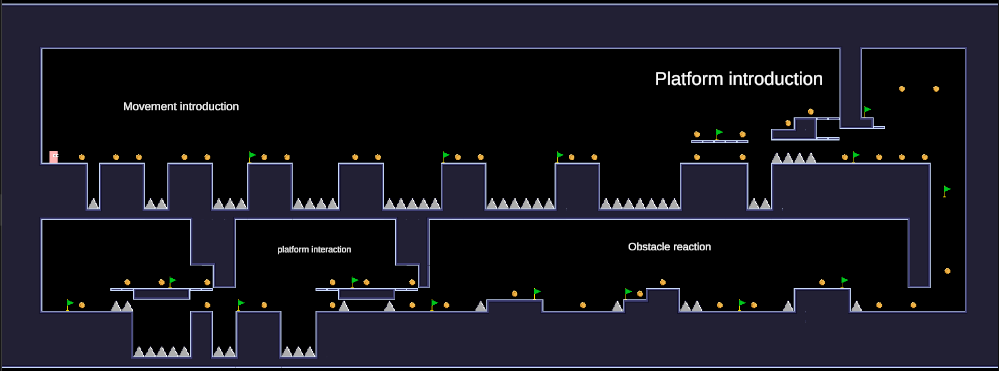
\includegraphics[width=10cm]{./Attachments/EnvironmentDesign.png}}
\caption{Environment training ground for the Ai}\label{fig:EnvironmentDesign}
\end{figure}
\subsection{Agent Actions}
Table \ref{tbl:Agent Actions Table} outlines the available actions for Player and Enemy agents. These actions simulate the gameplay mechanics and ensure that the AI can engage with the environment and other agents meaningfully.
\begin{table}[!h]
\caption{Agent Actions Table}\label{tbl:Agent Actions Table}
\begin{tabular}{|l|l|l|} \hline
& \textbf{Player Agent} & \textbf{Enemy Agent} \\ \hline
Actions & Walk and run & Walk and run \\ 
& Jump & Jump \\ 
& Attack (Melee) & Attack player (Melee)  \\ 
& Drop Down &  \\
& Dash &  \\ \hline
\end{tabular}
\end{table}
\subsubsection{Player Agent Actions}
\begin{itemize}
\item  \textbf{Walk and run:} Allows navigation of horizontal spaces.
\item  \textbf{Jump:} Essential for crossing gaps and reaching elevated platforms.
\item  \textbf{Attack (Melee):} Simulates combat mechanics where the player can engage with enemies or break objects.
\item  \textbf{Drop Down:} Enables traversal through one way platform accessing other places.
\item  \textbf{Dash:} Enables moving horizontally at a higher speed avoiding obstacles.
%\item  \textbf{Crouch:} Enables traversal through tight spaces or avoidance of overhead obstacles.%
\end{itemize}
\subsubsection{Enemy Agent}
\begin{itemize}
\item  \textbf{Walk and run:} Supports patrol or chase behaviors.
\item  \textbf{Jump:} Ensures enemies can traverse complex terrains.
\item  \textbf{Attack (Melee):} Adds combat mechanics, making the environment more dynamic.
%\item  \textbf{Crouch:} Enables traversal through tight spaces or avoidance of overhead obstacles.%
\end{itemize}
\subsection{Physics and Movement Constraints}
The game environment adheres to a realistic 2D physics system that governs movement dynamics. The agent’s movement system follows industry-standard platformer mechanics, ensuring consistency with human gameplay expectations.
\subsubsection{Movement Mechanics}
\begin{itemize}
\item  \textbf{Walking and Running:} The agent moves laterally within predefined speed limits.
\item  \textbf{Jumping:} The agent can jump with variable force depending on input duration.
\item  \textbf{Dashing:} A short burst movement in a direction, used for evasion or precise navigation.
\item  \textbf{Wall Interactions:} The agent can cling to or slide down walls, enabling wall jumps for vertical traversal.
\end{itemize}
\subsubsection{Collision and Interaction System}
The physics engine handles collisions and interactions between the agent and the environment using Unity’s built-in 2D physics system.
\begin{itemize}
\item  \textbf{Ground Detection:} Determines whether the agent is standing on a platform, affecting movement choices.
\item  \textbf{Hazard Detection:} Triggers damage events when colliding with harmful objects.
\item  \textbf{Enemy Interaction:} Enables combat-related decisions such as attacking or avoiding enemies.
\end{itemize}
By enforcing a consistent movement and interaction model, the environment ensures that the agent learns within realistic constraints, improving the generalizability of the trained AI.
\subsection{Environment Testing}
Before integrating the reinforcement learning model, rigorous environment testing is conducted to ensure the platformer world is functionally sound, scalable, and optimized for training.
\subsubsection{Functional Testing}
Functional tests verify that core game mechanics operate as intended:
\begin{itemize}
\item  \textbf{Movement Tests:} Ensuring the agent can walk, jump, dash, and interact with platforms correctly.
\item  \textbf{Collision Tests:} Verifying that the agent properly detects and responds to ground, walls, hazards, and enemies.
\item  \textbf{Camera Tests:} Confirming that the ML sprite system correctly renders simplified perception inputs.
\end{itemize}
\subsubsection{Performance Optimization}
Since reinforcement learning requires high-frequency environment interaction, performance optimizations are applied:
\begin{itemize}
\item  \textbf{Physics Simplification:} Reducing unnecessary physics calculations to improve simulation speed.
\item  \textbf{Memory Management:} Ensuring that ML sprite rendering and collision detection do not create excessive overhead.
\item  \textbf{Frame Rate Stability:} Maintaining consistent simulation speed to ensure uniform training conditions.
\end{itemize}
\subsubsection{Scalability Testing}
To ensure the environment remains adaptable for future projects, scalability tests evaluate:
\begin{itemize}
\item  \textbf{Level Size Variability:} Testing different map layouts to verify adaptability.
\item  \textbf{Enemy and Obstacle Density:} Measuring the impact of increased AI-controlled elements on performance.
\item  \textbf{Generalization Potential:} Ensuring that the AI can learn effectively in varied level designs without overfitting to a specific layout.
\end{itemize}
This testing process ensured that the game environment aligned with the project's objective of creating robust and reusable AI assets for game development.
\section{AI Algorithms and Models}
The artificial intelligence (AI) system in this project is designed to function as a reinforcement learning (RL) agent, capable of autonomously learning and executing platforming mechanics. The primary objective is to develop an adaptive AI agent that improves its performance through iterative learning. This agent is implemented using Unity ML-Agents, and training is conducted within the custom-built platformer game environment.
\subsection{Action Space and Decision-Making}
The action space defines the possible decisions the AI agent can take at any given time.\par
The following discrete actions are implemented in the platformer environment:\par
\begin{table}[!h]
\caption{Action Space Table}\label{tbl:Action Space Table}
\begin{tabular}{|l|l|} \hline
\textbf{Action} & \textbf{Description} \\ \hline
Move Left & Moves the agent left along the x-axis. \\ 
Move Right & Moves the agent right along the x-axis. \\ 
Jump & Initiates a jump if the agent is on solid ground. \\ 
Drop Down & Allows the agent to descend through one-way platforms. \\ 
Dash & Performs a short burst movement in the selected direction. \\ 
Attack & Executes a melee attack when enemies are in range. \\ \hline
\end{tabular}
\end{table}
The decision-making process is handled by the AI model, which outputs a probability distribution over possible actions at each time step. The agent selects an action based on learned policies, with an emphasis on maximizing future rewards.
\subsection{Reward and Penalty System}
The reinforcement learning model requires a reward function to guide learning. This function assigns positive rewards for desirable actions and penalties for suboptimal behavior.
\subsubsection{Player Agent Rewards and Penalties}
The Player Agent is primarily focused on completing levels and maximizing performance. The rewards and penalties assigned to the Player Agent are designed to incentivize behaviors that contribute to level progression, combat efficiency, and overall success.\par
\begin{table}[!h]
\caption{Player Agent Reward Table}\label{tbl:Player Agent Reward Table}
\begin{tabular}{|l|l|} \hline
\textbf{Action} & \textbf{Rewards} \\ \hline
Level Completion & +1000 \\ 
Enemy Defeated & +100 \\ 
Collecting Objective Items & +50 \\ 
Interact with Objectives & +20 \\ 
Exploring & +1 per new point reached \\ 
Falling or Hitting Hazards & -50 \\ 
Taking Damage from Enemy & -200 \\
Eliminated & -1000 \\ \hline
\end{tabular}
\end{table}
\subsubsection{Enemy Agent Rewards and Penalties}
The Enemy Agents are designed to create challenges for the Player Agent. Their behavior is shaped by rewards and penalties that encourage actions which counter the Player Agent's progress.\par
\begin{table}[!h]
\caption{Enemy Agent Reward Table}\label{tbl:Enemy Agent Reward Table}
\begin{tabular}{|l|l|} \hline
\textbf{Action} & \textbf{Rewards} \\ \hline
Player Damaged & +100  \\ 
Chasing Player & +5  for every period of time chasing player \\ 
Survival Time & +1 for every period of time survived \\
Falling or Hitting Hazards & -50 \\ 
Eliminated & -200 \\ \hline
\end{tabular}
\end{table}
This reward system is fine-tuned iteratively to ensure that the AI develops efficient and strategic movement patterns without exploiting rewards through unintended behaviors.\par
\subsection{Agent Perception and Observations}
To facilitate intelligent decision-making, the AI agent perceives the environment through a structured observation space, eliminating reliance on raycasting and instead leveraging a dedicated agent camera with simplified ML sprites. This approach mirrors human vision-based gameplay and enhances the interpretability of learned behaviors.
\subsubsection{Observation Space and State Representation}
The agent receives structured inputs that define its state and surroundings:\par
\textbf{Positional and Movement Awareness}
\begin{itemize}
\item  \textbf{Current position} within the game world.
\item  \textbf{Grounded status} \texttt{IsGrounded}  determines if the agent is standing on solid ground.
\item  \textbf{Jumping status} \texttt{IsJumping}  determines if the agent is jumping or in mid air from the ground.
\item  \textbf{Dashing status} \texttt{IsDashing}  determines if the agent is in the dashing state.
\item  \textbf{Dropping status} \texttt{IsDropping}  determines if the agent is dropping from a one way platform.
\item  \textbf{On-wall status} \texttt{IsOnWall}  determines if the agent is on the wall, available for wall related actions.
\item  \textbf{Wall-jumping status} \texttt{IsWallJumping}  determines if the agent is jumping off from a wall.
\item  \textbf{Facing direction} \texttt{IsFacingRight}  determines if the agent is facing right or left.
\end{itemize}
\textbf{Environmental Awareness}
\begin{itemize}
\item  Proximity to enemies, hazards, or collectibles.
\item  \textbf{Checkpoint status:} tracks progress within the level.
\item  \textbf{Health and damage state:} monitors the agent’s survival status.
\end{itemize}
\subsubsection{Camera-Based Perception and ML Sprite System}
A unique aspect of this project is the decision to replace traditional raycasting techniques with a dedicated agent camera. This approach mimics human player perception, where decision-making is based on visible elements rather than invisible proximity checks or abstract sensor inputs.
To implement this, the game utilizes a dual-layer rendering system:
\begin{itemize}
\item  \textbf{Primary Camera (Player Perspective):}
The main camera, which is responsible for rendering the actual game world as seen by the player. This includes fully detailed textures, lighting effects, UI elements, and all in-game objects categorized into specific layers such as Ground, Enemy, Prize, Checkpoint, etc.
\begin{figure}[!h]
\centering
\fbox{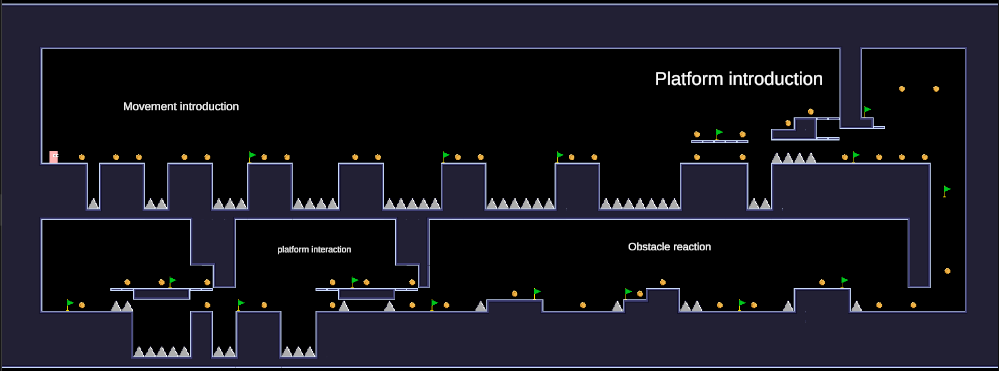
\includegraphics[width=10cm]{./Attachments/EnvironmentDesign.png}}
\caption{Player perspective}\label{fig:PlayerPers}
\end{figure}
\item  \textbf{Agent Camera (AI Perspective):}
A separate camera dedicated to the AI agent, rendering a simplified version of the game world. This camera ignores visual effects and detailed textures, instead utilizing a distinct ML sprite system composed of minimalistic geometric representations of in-game objects.
\begin{figure}[!h]
\centering
\fbox{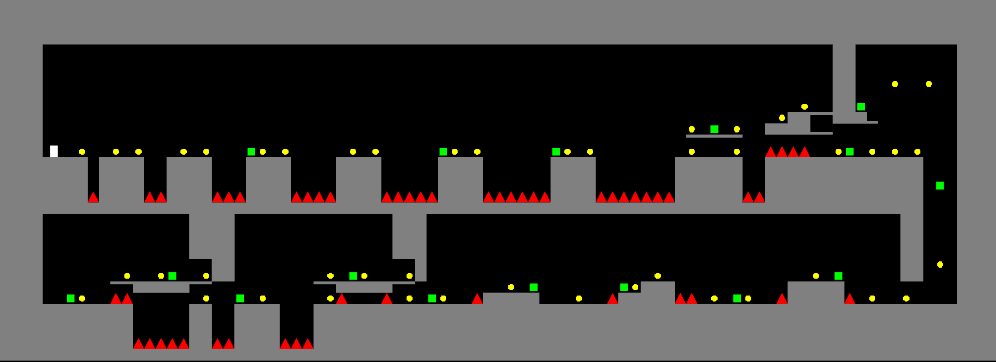
\includegraphics[width=10cm]{./Attachments/AiPerspective.png}}
\caption{AI perspective}\label{fig:AIPers}
\end{figure}
\end{itemize}
\textbf{ML Sprite Classification System}\par
Each object in the environment is assigned a secondary ML sprite, which is rendered exclusively for the agent camera. These ML sprites are categorized into distinct layer masks and follow a predefined color-coded classification system to provide the AI with structured, interpretable visual data.\par
The classification scheme is as follows:\par
\begin{table}[!h]
\caption{Sprite Color Code Table}\label{tbl:Sprite Color Code Table}
\begin{tabular}{|l|l|l|} \hline
\textbf{Color} & \textbf{Meaning} & \textbf{Hex Code} \\ \hline
White & Player & \texttt{\#FFFFFF} \\ 
Red & Hazards (traps, spikes) & \texttt{\#FF0000} \\ 
Magenta & 	Enemies (attackable entities) & \texttt{\#FF00FF}  \\ 
Green & Goals (checkpoints, exits) & \texttt{\#00FF00} \\ 
Yellow & Collectibles (coins) & \texttt{\#FFFF00} \\ 
Blue & Attacking hitboxes & \texttt{\#0000FF} \\ 
Gray & Ground (solid platforms) & \texttt{\#808080} \\ \hline
\end{tabular}
\end{table}
Through this system, the agent perceives objects in an abstract yet structured manner, focusing only on relevant gameplay elements rather than unnecessary graphical details. This enables a highly extensible framework where additional layers or object categories can be introduced seamlessly by developers integrating this AI into their own projects.
\section{Training Process and Optimization}
The training process of the AI agent follows a structured pipeline designed to optimize learning efficiency and ensure convergence towards an optimal policy. This process consists of data collection, policy network updates, curriculum learning strategies, and performance evaluation metrics. By leveraging reinforcement learning (RL) principles, particularly policy optimization methods, the AI progressively refines its ability to navigate the platformer environment.
\subsection{Data Collection and Experience Buffer}
During training, the AI agent interacts with the environment and records state-action-reward sequences. These experiences are stored in a replay buffer, which helps the agent learn by analyzing past interactions.\par
\subsubsection{Experience Replay and Data Storage}
Unlike traditional online learning, where updates occur immediately after each action, experience replay (as employed in off-policy learning techniques) allows the AI agent to learn from a diverse set of past interactions. This enhances sample efficiency and reduces training instability by preventing excessive bias toward recent experiences.\par The data collection process consists of:
\begin{itemize}
\item \textbf{State Observations:} Capturing spatial and contextual information from the environment at each timestep.
\item \textbf{Action Selection:} The policy network predicts the most suitable action based on past experiences.
\item \textbf{Reward Assignment:} The agent receives feedback (reward or penalty) based on its action.
\item \textbf{Storage in Replay Buffer:} The tuple (state, action, reward, next state) is stored in memory.
\item \textbf{Batch Sampling for Training:} A mini-batch of past experiences is selected for policy updates.
\end{itemize}
\subsection{Policy Network Training}
he AI agent employs a neural network-based policy model, where policy parameters are updated iteratively using gradient-based optimization techniques. The training process consists of several key components:
\begin{itemize}
\item  \textbf{Collecting gameplay experiences:} The AI agent performs actions in the environment.
\item  \textbf{Evaluating rewards:} The system calculates cumulative rewards for different strategies.
\item  \textbf{Updating the policy:} The AI refines its decision-making using policy gradient updates.
\end{itemize}
\subsection{Curriculum Learning Approach}
To facilitate structured learning, a curriculum-based training strategy is employed, wherein training difficulty is gradually increased as the AI model improves. This approach enables more stable learning and prevents the agent from being overwhelmed by complex tasks in the early stages.\par
The curriculum is structured into four phases:
\begin{itemize}
\item  \textbf{Phase 1: Basic Movement Training:} The agent learns fundamental mechanics such as walking, jumping, and dashing in an obstacle-free environment.
\item  \textbf{Phase 2: Platforming Challenges:} The environment introduces gaps, moving platforms, and elevation changes to refine traversal skills.
\item  \textbf{Phase 3: Combat Scenarios:} The agent encounters dynamic enemies, learning attack patterns and defensive maneuvers.
\item  \textbf{Phase 4: Full-Level Training:} The AI is trained in fully designed levels, requiring mastery of all mechanics to complete objectives.
\end{itemize}
\subsection{Performance Metrics and Convergence}
The efficiency of training is evaluated using key performance indicators (KPIs) that measure learning progress and policy effectiveness.\par
\subsubsection{Cumulative Reward Trend}
\begin{itemize}
\item  Tracks the total reward accumulated per episode.
\item  Indicates whether the agent is improving over time.
\item  A consistently increasing reward trend suggests successful learning.
\end{itemize}
\subsubsection{Episode Length}
\begin{itemize}
\item  Measures the duration of each playthrough.
\item  Shorter episodes in earlier training stages may indicate suboptimal policies (e.g., frequent deaths).
\item  As training progresses, longer episode lengths suggest improved survival and decision-making.
\end{itemize}
\subsubsection{Success Rate}
\begin{itemize}
\item  Defined as the percentage of episodes in which the agent successfully reaches level objectives.
\item  A threshold success rate (e.g., 95\%) can be set to determine when training should be finalized.
\end{itemize}
\subsubsection{Training Convergence}
Training is considered complete once performance metrics stabilize, indicating that additional training no longer significantly improves the policy.\par Convergence is monitored using:\par
\begin{itemize}
\item  \textbf{Policy Entropy:} Ensuring the model does not become overconfident in suboptimal actions.
\item  \textbf{Variance in Success Rate:} Stability in success rate across multiple test runs.
\item  \textbf{Generalization Testing:} Evaluating the AI on unseen levels to verify adaptability.
\end{itemize}

\section {AI Implementation and Packaging}
The successful deployment of the trained AI model within a game development environment necessitates a structured approach to integration, optimization, and packaging. This process ensures that the AI agent functions efficiently within the Unity-based platformer while also being modular and reusable for future projects. Additionally, the AI system is designed to be packaged as a standalone asset that developers can easily integrate into similar games without requiring extensive modifications.\par
This section outlines the methodology for embedding the AI model into the game engine, optimizing its execution, setting up a dual-rendering system for enhanced perception, and packaging it as a shareable Unity asset.\par
\subsection{Integration of the Trained AI Model}
After the reinforcement learning model has been trained and validated, it is integrated into the Unity project for real-time inference. The AI must be able to process environmental inputs and execute actions effectively while maintaining computational efficiency.
\subsubsection{Loading and Utilizing the Trained Model}
The trained model is exported as a \texttt{.onnx} file, a format compatible with Unity’s ML-Agents inference system.\par The steps for incorporating the model into the game are as follows:\par
\begin{itemize}
\item  \textbf{Model Importion}
\begin{itemize}
\item  The \texttt{.onnx} model file is placed into the Unity project’s Assets directory.
\item  Unity’s Behavior Parameters component is configured to reference the model.
\end{itemize}
\item  \textbf{Agent Configuration}
\begin{itemize}
\item  The AI agent is modified to switch from training mode to inference mode.
\item  The model receives observations from the environment and produces action outputs in real time.
\end{itemize}
\item  \textbf{Testing and Validation}
\begin{itemize}
\item  The AI’s performance is validated within a controlled game scenario.
\item  Debugging tools are used to monitor decision-making processes and adjust parameters as needed.
\end{itemize}
\end{itemize}
\subsection{Dual-Rendering System for Agent Perception}
To enhance the AI’s perception of the game environment, a dual-rendering system is implemented, allowing the agent to interpret its surroundings using a dedicated perception layer distinct from the player's visual representation. This approach improves object recognition and state representation, optimizing learning efficiency and decision-making accuracy.
\subsubsection{Design and Implementation}
\begin{itemize}
\item  \textbf{Primary Camera (Player View)}
\begin{itemize}
\item  This camera renders the standard game environment for the player.
\item  Traditional visual element layers, including textures, lighting, and UI elements, are rendered with this camera.
\end{itemize}
\item  \textbf{Secondary Camera (Agent Perception View)}
\begin{itemize}
\item  A separate, hidden camera renders a simplified version of the environment specifically for the AI.
\item  Objects are color-coded as provided in the table \ref{tbl:Sprite Color Code Table} instead of textured, reducing unnecessary complexity.
\item  Dynamic elements such as enemies and hazards are highlighted distinctly.
\end{itemize}
\item  \textbf{Integration with ML-Agents}
\begin{itemize}
\item  The AI model receives input from the perception camera rather than the full game scene.
\item  Observation preprocessing converts the camera feed into a structured tensor representation.
\end{itemize}
\end{itemize}
\subsubsection{Advantages of the Dual-Rendering System}
\begin{itemize}
\item  \textbf{Reduces Unnecessary Complexity:} The AI perceives only relevant elements, improving training efficiency.
\item  \textbf{Standardizes Input Data:} Ensures consistency across different game levels or environments.
\item  \textbf{Optimizes Learning Speed:} Simplifies object recognition, allowing the model to generalize more effectively.
\end{itemize}
\subsection{Modular AI System for Reusability}
To ensure adaptability across multiple projects, the AI system follows a modular design, enabling easy integration with different platformer environments. The key components include:
\begin{itemize}
\item  \textbf{ActionModule:} Centralizes AI interactions with the game, allowing for customization of available actions (e.g., jumping, attacking).
\item  \textbf{Customizable Observations:} The AI’s input space can be modified based on environmental conditions.
\item  \textbf{Configurable Reward System:} Developers can fine-tune rewards to optimize learning outcomes.
\item  \textbf{Flexible Behavior Parameters:} AI response time, exploration rate, and decision frequency can be adjusted dynamically.
\end{itemize}
\subsection{Packaging the AI as a Reusable Unity Asset}
To facilitate widespread adoption, the AI system is packaged as a Unity asset bundle, allowing developers to easily import and configure the AI within their own projects. The packaging process follows structured guidelines to ensure compatibility and ease of use.
\subsubsection{Asset Bundling and Exportation}
\begin{itemize}
\item  The AI scripts, model files, and configuration settings are structured into a self-contained Unity package.
\item  Dependencies such as ML-Agents are documented to streamline integration.
\item  A standardized folder structure is maintained to enhance clarity.
\end{itemize}
\subsubsection{Documentation and User Guide}
\begin{itemize}
\item  A \texttt{README.md} file provides quick-start instructions.
\item  A detailed PDF manual explains AI setup, customization, and troubleshooting.
\item  Code examples illustrate how to modify AI behaviors for specific game mechanics.
\end{itemize}
\subsubsection{Version Control and Distribution}
\begin{itemize}
\item  The AI package is versioned, with changelogs detailing improvements.
\item  Distribution options include GitHub, Unity Asset Store, and private repositories.
\item  Developers are encouraged to contribute enhancements to ensure long-term maintainability.
\end{itemize}
%%%%%%%%%%%%%%%%%%%%%%%%%%%%%%%%%%%%%%%%%%%%%%%%%%%%%%%%%%%%%%
%%%%%%%%%%%%%%%%%%%% Experiments %%%%%%%%%%%%%%%%%%%%%%%%%%%%%
%%%%%%%%%%%%%%%%%%%%%%%%%%%%%%%%%%%%%%%%%%%%%%%%%%%%%%%%%%%%%%%
\chapter{Results and Current AI Capabilities}
This chapter presents the current state of the AI system in the wake of training and implementation. In-depth consideration is given to the performance of the AI within the established environment in terms of ability to navigate, interact with the game elements, and make decisions through the reinforcement learning framework. The results portray the present-day functionality of the system without speculation regarding future developments or improvements.
\section{Overview of Accomplishments}
\subsection{Movement and Navigation}
After carefully training for an extensive period using the PPO reinforcement learning algorithm, the AI agent has become capable of fully controlling itself in the platformer's environment. With a reliably functioning walking, jumping, and descent mechanism, the agent can drop straight from one-way platforms. As a result of iterative reinforcement learning, the model knows the optimal paths of movement by which he could traverse efficiently without much delay, avoid an obstruction, and come to certain destinations within the level. The AIs keep both exploration and efficient across-the-board movement and minimizing downside-avoiding turns while remaining adaptive to different terrains.
\begin{figure}[!h]
\centering
\fbox{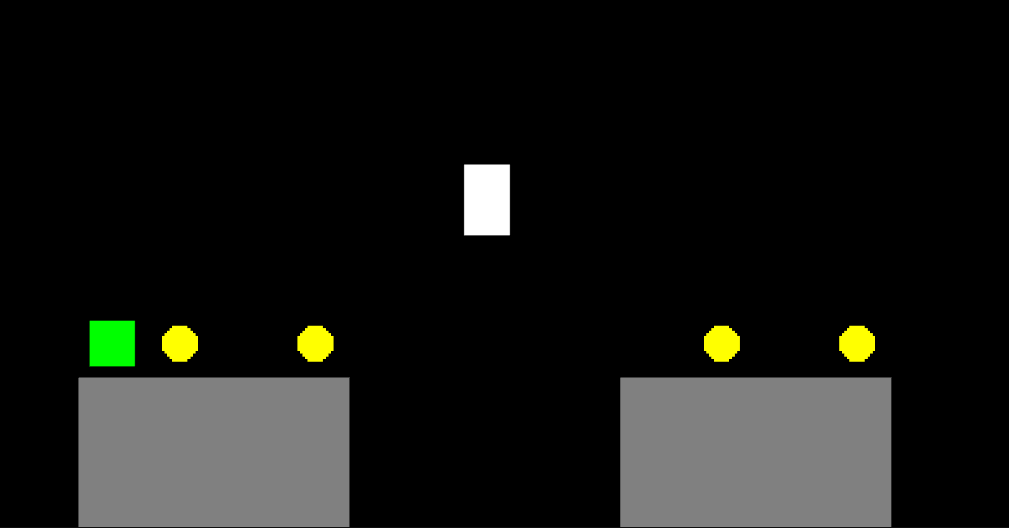
\includegraphics[width=10cm]{./Attachments/AiJump.png}}
\caption{AI bot hopping from ground to another.}\label{fig:AIJump}
\end{figure}
\newpage
\subsection{Interaction with Collectibles and Obstacles}
The AI agent acquired knowledge in the interaction of collecting objects and environmental obstacles. It has also learned to identify and prioritize collecting objects, such as coins, adjust its movement to them, and optimize the reward received from them. The improvement of avoidance by hazardous events has demonstrated the ability to recognize penalty-inducing-threshold objects and determine trajectory modification. The ability to run these behaviors accurately signifies that the AI can consistently complete test runs in the environment without failing in excess.
\begin{figure}[!h]
\centering
\fbox{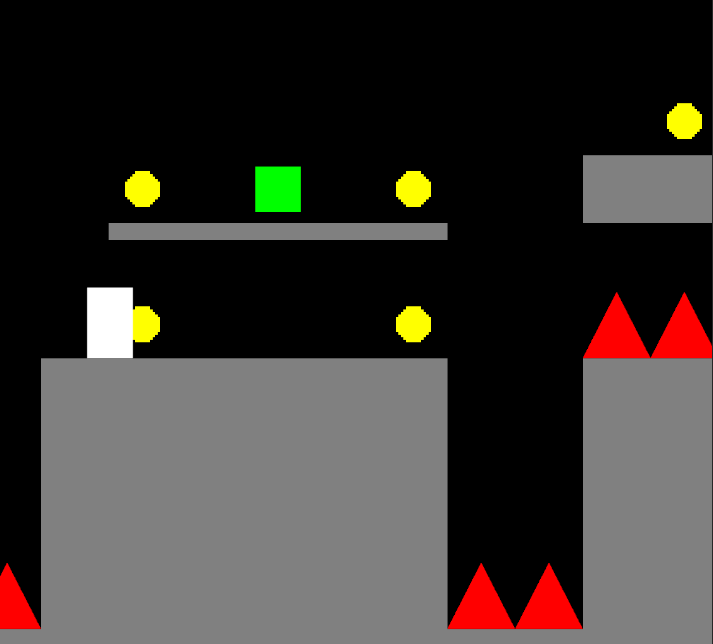
\includegraphics[width=10cm]{./Attachments/AiInteract.png}}
\caption{AI bot interacting collectible and obstacles.}\label{fig:AIInt}
\end{figure}
\subsection{Combat and Adaptive Behavior}
As a consequence, the developmental capacities of AI now depend on movement and interaction with other worlds; combat mechanics have not been integrated into the reinforcement learning architecture as yet, and AI does not know how to perform attack sequences or enemy encounters. As a result, the present section does not contain any results for adversarial behavior or combat-related decision-making. The existing implementation continues to be focused on traversal and interactions with the environment as currently foundation lines for future use extensions in terms of functionalities.
\section{Training Performance Metrics}
\subsection{The Reward Functions Performing}
The Reinforcement learning algorithms have exhibited good and stable trends of reward acquisition from one training cycle to the next. History shows improvements in increments of reward as occurrences of sub-optimal or penalty behavior decline. Thus, the agent has managed to utilize positive reinforcement, indicating the successful design of the reward function to facilitate movement and interaction optimally.
\subsection{Convergence and Stability}
Evidence of training convergence has been through stabilization in performance over many episodes. The first few phases of training revealed very high variance in agent behavior performance in making decisions and severe penalties. However, the learning model, after training over a sufficient number of epochs, has reduced the performance fluctuation, indicating stable learning and lesser dependence on exploratory randomness. The convergence of the policy indicates a successful imprinting of an optimal decision-making structure within the agent by the training process.
\subsection{Evaluation of Training Efficiency}
The evaluation of training efficiency was through policy improvement rate and reduction of superfluous movements. The learning curve of the AI clearly indicates the improvement as it refrained from making unnecessary movements early on before improving the strategy. Other training efficiencies have been enhanced by tuning hyperparameters and distributing rewards, making learning focused and effective in computational use.
\section{AI Behavior in Environment training ground}
\subsection{Behavior Under Different Level Designs}
Varieties of platform layouts offered opportunity to review generalization properties of the AI model. Test results illustrate the versatility of the trained policy across structurally similar environments. High navigation and interaction performances are sustained. The AI can adapt to different setups without retraining as long as the key level design principles stay within the threshold defined by the training environment.
\subsection{Response to Dynamic Obstacles}
The AI shows a degree of flexibility in interacting with moving obstacles or hazards in the environment, whereby learned avoidance allows the agent to detect and circumvent moving threats with adjustments to time and trajectory accordingly. The steady successful performance on avoidance would suggest that reinforcement learning has encoded a decisional process for hazard avoidance. 
\subsection{Efficacy in Collectible Acquisition}
In tasks where collectible objects were tested in the environment, the AI was observed to optimize paths when seeking maximal reward. This reliance was mostly without detours as the agent preferred the path of least resistance toward collectible objects, following the decision patterns as defined by the reinforcement structure. Thus, the AI's consistent behavior in achieving successful item collection while avoiding hazards proves its risky behavior and reward calculations in a game.
\section{Implementation and Integration of AI}
\subsection{AI Integration in the Unity Environment}
The integrated AI model works fully in the Unity platformer game in real time. Transitioning from simulated training environments to real-time execution appeared completely uneventful, with the AI behaving exactly as it was supposed to, following the learned patterns from training data. This has been made possible by synchronization using the ML-Agents package in Unity so that the AI decision-making can continuously interact with the physics of the game and the game world.
\subsection{AI Perception and a Dual-Render Environment Setup}
The dual-render environment setup allows the AI perception system to distinguish between the in-game elements. It enables the agent to structure information on the environment so that the decision-making mechanism correctly identifies relevant objects, such as the platform, obstacles, and collectibles. A rendering-based system increases the spatial awareness of the AI and hence the contextually relevant actions that can be taken.
\subsection{Modularity and Reusability in Implementation}
The AI system is designed as a modular system to promote reusability across projects. Movement controllers, reward functions, and decision- making modules are key components that can be adjusted to new environments in the implementation without requiring extensive reconfiguration. Thus, this modular approach enhances the AI's suitability to even more varied platformer game projects, which are intended to become an AI reusable asset.
\section{Summary of Current AI Capabilities}
The AI system is now competent in the movement, navigation, and interaction of a platformer game. It has shown convergence in learning which is stable, effective awareness of its environment, and generalized behavior across different level designs. Although combat is not yet in use, the current implementation offers a firm groundwork for extended AI development in platformer games. The reinforcement-learning framework has fostered agent behavior that is conducive to the free navigation and interaction of game elements in a structured and goal-directed manner.


%%%%%%%%%%%%%%%%%%%%%%%%%%%%%%%%%%%%%%%%%%%%%%%%%%%%%%%%%%%%%%%
%%%%%%%%%%%%%%%%%%%% Conclusions %%%%%%%%%%%%%%%%%%%%%%%%%%%%%
%%%%%%%%%%%%%%%%%%%%%%%%%%%%%%%%%%%%%%%%%%%%%%%%%%%%%%%%%%%%%%%
\chapter{Conclusions}

 \begin{figure}[!h]
\caption{This is how you mention when figure come from internet  \href{https://www.google.com} {https://www.google.com}}\label{fig:x1}
\end{figure}

This chapter is optional for proposal and progress reports but 
is required for the final report.

THIS IS AN EXAMPLE. ALL SECTIONS BELOW ARE OPTIONAL. PLEASE CONSULT YOU ADVISOR AND DESIGN YOUR OWN SECTION

\emph{\textthai{หัวข้อต่าง ๆ ในแต่ละบทเป็นเพียงตัวอย่างเท่านั้น หัวข้อที่จะใส่ในแต่ละบทขึ้นอยู่กับโปรเจคของนักศึกษาและอาจารย์ที่ปรึกษา}}

\section{Problems and Solutions}
State your problems and how you fixed them.

\section{Future Works}
What could be done in the future to make your projects better.

%%%%%%%%%%%%%%%%%%%%%%%%%%%%%%%%%%%%%%%%%%%%%%%%%%%%%%%%%%%%%%%
%%%%%%%%%%%%%%%%%%%% Bibliography %%%%%%%%%%%%%%%%%%%%%%%%%%%%%
%%%%%%%%%%%%%%%%%%%%%%%%%%%%%%%%%%%%%%%%%%%%%%%%%%%%%%%%%%%%%%%

%%%% Comment this in your report to show only references you have
%%%% cited. Otherwise, all the references below will be shown.
%\nocite{*}
%% Use the kmutt.bst for bibtex bibliography style 
%% You must have cpe.bib and string.bib in your current directory.
%% You may go to file .bbl to manually edit the bib items.

% Sept, 2021 by Thanin
% improve url breaks to prevent unnecessary big white spaces in some cases
\makeatletter
\g@addto@macro{\UrlBreaks}{\UrlOrds}
\makeatother
% 

\bibliographystyle{kmutt}
\bibliography{string,cpe}

%%%%%%%%%%%%%%%%%%%%%%%%%%%%%%%%%%%%%%%%%%%%%%%%%%%%%%%%%%%%%%%
%%%%%%%%%%%%%%%%%%%%%%%% Appendix %%%%%%%%%%%%%%%%%%%%%%%%%%%%%
%%%%%%%%%%%%%%%%%%%%%%%%%%%%%%%%%%%%%%%%%%%%%%%%%%%%%%%%%%%%%%%
\appendix{First appendix title}
\noindent{\large\bf Put appropriate topic here} \\

This is where you put hardware circuit diagrams, detailed experimental data in tables or source codes, etc.. \\ \bigskip

 \begin{figure}[!h]
\caption{This is the figure x11 \href{https://www.google.com} {https://www.google.com}}\label{fig:x1}
\end{figure}

This appendix describes two static allocation methods for fGn (or fBm)
traffic. Here, $\lambda$ and $C$ are respectively the traffic arrival
rate and the service rate per dimensionless time step. Their unit are
converted to a physical time unit by multiplying the step size
$\Delta$. For a fBm self-similar traffic source,
Norros~\cite{norros95} provides its EB as
\begin{equation}\label{eq:norros}
  C = \lambda + (\kappa(H)\sqrt{-2\ln\epsilon})^{1/H}a^{1/(2H)}x^{-(1-H)/H}\lambda^{1/(2H)}
\end{equation}
where $\kappa(H) = H^H(1-H)^{(1-H)}$. Simplicity in the calculation is
the attractive feature of (\ref{eq:norros}).

The MVA technique developed in~\cite{kim01} so far provides the most
accurate estimation of the loss probability compared to previous
bandwidth allocation techniques according to simulation results.
Consider a discrete-time queueing system with constant service rate
$C$ and input process $\lambda_n$ with $\mathbb{E}\{\lambda_n\} =
\lambda$ and $\mathrm{Var}\{\lambda_n\} = \sigma^2$.  Define $X_n \equiv
\sum_{k=1}^n \lambda_k - Cn$.  The loss probability due to the MVA
approach is given by
\begin{equation}\label{eq:loss_mva}
  \varepsilon \approx \alpha e^{-m_x/2}
\end{equation}
where
\begin{equation}\label{eq:mx}
m_x = \min_{n \geq 0} \frac{((C-\lambda)n + B)^2}{\mathrm{Var}\{X_n\}} =
\frac{((C-\lambda)n^\ast + B)^2}{\mathrm{Var}\{X_{n^{\ast}}\}}
\end{equation} 
and 
\begin{equation}\label{eq:alpha}
  \alpha =
  \frac{1}{\lambda\sqrt{2\pi\sigma^2}}\exp\left(\frac{(C-\lambda)^2}{2\sigma^2}\right)
  \int_C^\infty (r-C)\exp\left(\frac{(r-\lambda)^2}{2\sigma^2}\right)\, dr
\end{equation}
For a given $\varepsilon$, we numerically solve for $C$ that satisfies
(\ref{eq:loss_mva}). Any search algorithm can be used to do the task.
Here, the bisection method is used.  

Next, we show how $\mathrm{Var}\{X_n\}$ can be determined.  Let
$C_{\lambda}(l)$ be the autocovariance function of $\lambda_n$.  The
MVA technique basically approximates the input process $\lambda_n$
with a Gaussian process, which allows $\mathrm{Var}\{X_n\}$ to be
represented by the autocovariance function.  In particular, the
variance of $X_n$ can be expressed in terms of $C_{\lambda}(l)$ as
\begin{equation}
  \mathrm{Var}\{X_n\} = nC_{\lambda}(0) + 2\sum_{l=1}^{n-1} (n-l)C_{\lambda}(l)
\end{equation} 
Therefore, $C_{\lambda}(l)$ must be known in the MVA technique, either
by assuming specific traffic models or by off-line analysis in case of
traces.  In most practical situations, $C_{\lambda}(l)$ will not be
known in advance, and an on-line measurement algorithm developed
in~\cite{eun01} is required to jointly determine both $n^\ast$ and
$m_x$. For fGn traffic, $\mathrm{Var}\{X_n\}$ is equal to $\sigma^2
n^{2H}$, where $\sigma^2 = \mathrm{Var}\{\lambda_n\}$, and we can find
the $n^\ast$ that minimizes (\ref{eq:mx}) directly. Although $\lambda$
can be easily measured, it is not the case for $\sigma^2$ and $H$.
Consequently, the MVA technique suffers from the need of prior
knowledge traffic parameters.


%%%%%%%%%%%%%%%%%%%%%%%%%%%%%%%%%%%%%%%%%%%%%%%%%%%%%%%%%%
%%%%%%%%%%%%%%% The 2nd appendix %%%%%%%%%%%%%%%%%%%%%%%%%%
%%%%%%%%%%%%%%%%%%%%%%%%%%%%%%%%%%%%%%%%%%%%%%%%%%%%%%%%%%
\appendix{Second appendix title}
\noindent{\large\bf Put appropriate topic here} \\


 \begin{figure}[!h]
\caption{This is the figure x11 \href{https://www.google.com} {https://www.google.com}}\label{fig:x1}
\end{figure}

Next, we show how $\mathrm{Var}\{X_n\}$ can be determined.  Let
$C_{\lambda}(l)$ be the autocovariance function of $\lambda_n$.  The
MVA technique basically approximates the input process $\lambda_n$
with a Gaussian process, which allows $\mathrm{Var}\{X_n\}$ to be
represented by the autocovariance function.  In particular, the
variance of $X_n$ can be expressed in terms of $C_{\lambda}(l)$ as
\begin{equation}
  \mathrm{Var}\{X_n\} = nC_{\lambda}(0) + 2\sum_{l=1}^{n-1} (n-l)C_{\lambda}(l)
\end{equation} 

\noindent{\large\bf Add more topic as you need} \\

Therefore, $C_{\lambda}(l)$ must be known in the MVA technique, either
by assuming specific traffic models or by off-line analysis in case of
traces.  In most practical situations, $C_{\lambda}(l)$ will not be
known in advance, and an on-line measurement algorithm developed
in~\cite{eun01} is required to jointly determine both $n^\ast$ and
$m_x$. For fGn traffic, $\mathrm{Var}\{X_n\}$ is equal to $\sigma^2
n^{2H}$, where $\sigma^2 = \mathrm{Var}\{\lambda_n\}$, and we can find
the $n^\ast$ that minimizes (\ref{eq:mx}) directly. Although $\lambda$
can be easily measured, it is not the case for $\sigma^2$ and $H$.
Consequently, the MVA technique suffers from the need of prior
knowledge traffic parameters. 





\end{document}
